\documentclass[a4paper]{article}
\usepackage[utf8]{inputenc}
\usepackage[russian]{babel}
\usepackage[T2]{fontenc}
\usepackage[warn]{mathtext}
\usepackage{graphicx}
\usepackage{amsmath}
\usepackage{floatflt}
\usepackage{amssymb}
\usepackage[left=20mm, top=20mm, right=20mm, bottom=20mm, footskip=10mm]{geometry}


\graphicspath{ {images/} }
\usepackage{multicol}
\setlength{\columnsep}{2cm}


\begin{document}

\begin{titlepage}
	\centering
	\vspace{5cm}
	{\scshape\LARGE Московский физико-технический институт \par}
	\vspace{4cm}
	{\scshape\Large Лабораторная работа \par}
	\vspace{1cm}
	{\huge\bfseries Компьютерная сцинтилляционная $\gamma$-спектрометрия \par}
	\vspace{1cm}
	\vfill
\begin{flushright}
	{\large выполнили студены 653 группы ФФКЭ}\par
	\vspace{0.3cm}
	{\LARGE Карпова Татьяна} \par
	{\LARGE Агафонов Владислав} \par

\end{flushright}
	

	\vfill

% Bottom of the page
	Долгопрудный, 2018 г.
\end{titlepage}

\section{Цель работы}
Снять и исследовать спектры излучения различных источников, характеризовать различные пики в спектрах радиоактивных веществ.

\section{В работе используются:}
\begin{itemize}
    \item сцинтиллятор
    \item ФЭУ
    \item предусилитель импульсов
    \item высоковольтный блок питания для ФЭУ
    \item АЦП
    \item компьютер.
\end{itemize}

\section{Теоретические положения}
\textbf{Фотоэффект} - это процесс взаимодействия гамма-кванта с электроном, связанным с атомом, при котором электрону передается вся энергия гамма-кванта. При этом электрону сообщается кинетическая энергия $T_e=E_\gamma-I_i$, где $E_\gamma$ -- энергия гамма-кванта, $I_i$ -- потенциал ионизации $i$-той оболочки атома. Фотоэффект особенно существенен для тяжелых веществ, где он идет с заметной вероятностью даже при высоких энергиях гамма-квантов. В легких веществах фотоэффект становится заметен лишь при относительно небольших энергиях гамма-квантов.  \par
\textbf{Эффект Комптона} - это упругое рассеяние фотона на свободном электроне, сопровождающееся изменением длины волны фотона. Максимальная энергия образующихся комптоновских электронов соответствует рассеянию гамма-квантов на $180^\circ$ и равна
\begin{equation}
E_{\max}=\frac{\eta\omega}{1+\frac{mc^2}{2\eta\omega}}.
\end{equation}
\textbf{Процесс образования электрон-позитронных пар.}
При достаточно высокой энергии гамма-кванта наряду с фотоэффектом и эффектом Комптона может происходить третий вид взаимодействия гамма-квантов с веществом -- образование электрон-позитронных пар. Процесс образования пар не может происходить в пустоте, так как в этом случае не выполняются законы сохранения энергии и импульса. В присутствии ядра или электрона процесс образования пары гамма-квантов возможен, так как можно распределить энергию и импульс гамма-кванта между тремя частицами без противоречия с законами сохранения. При этом если процесс образования пары идет в кулоновском поле ядра или протона, то энергия образующегося ядра отдачи оказывается весьма малой, так что пороговая энергия гамма-кванта $E_0$, необходимая для образования пары, практически совпадает с удвоенной энергией покоя электрона $E_0\cong 2mc^2=1.022$ МэВ.\par
Появившийся в результате процесса образования пар электрон свою энергию на ионизацию среды. Таким образом, вся энергия электрона остается в детекторе. Позитрон будет двигаться до тех пор, пока практически не остановится, а затем аннигилирует с электроном среды, в результате чего появятся два гамма-кванта. Т.е., кинетическая энергия позитрона также останется в детекторе. Далее возможны три варианта развития событий:
\begin{enumerate}
\item оба родившихся гамма-кванта не вылетают из детектора, и тогда вся энергия первичного гамма-кванта останется в детекторе, а в спектре появится пик с $E=E_{\gamma}$;
\item один из родившихся гамма-квантов покидает детектор, и в спектре появляется пик, соответствующий энергии $E=E_{\gamma}-E_0$, где $E_0=mc^2=511$ кэВ;
\item оба родившихся гамма-кванта покидают детектор, и в спектре появляется пик, соотвествующий энергии $E=E_{\gamma}-2E_0$, где $2E_0=2mc^2=1022$ кэВ.
\end{enumerate}
Таким образом, любой спектр, получаемый с помощью гамма-спектрометра, описывается несколькими компонентами, каждая из которых связана с определенным физическим процессом. Как описано выше, основными физическими процессами взаимодействия гамма-квантов с веществом является фотоэффект, эффект Комптона и образование электрон-позитронных пар, и каждый из них вносит свой вклад в образование спектра. Помимо этих процессов, добавляется \textit{экспонента}, связанная с наличием фона, \textit{пик характеристического излучения}, возникающий при взаимодействии гамма-квантов с окружающим веществом, а также \textit{пик обратного рассеяния}, образующийся при энергии квантов $E_{\gamma}\gg mc^2/2$ в результате рассеяния гамма-квантов на большие углы на материалах  конструктивных элементов детектора и защиты. Положение пика обратного рассеяния определяется по формуле:
\begin{equation}
E_{\text{обр}}=\frac{E}{1+2E/mc^2},
\label{eq:Ereverse}
\end{equation}
где $E$ -- энергия фотопика.\par
\paragraph{Энергетическое разрешение спектрометра.} Даже при поглощении частиц с одинаковой энергией амплитуда импульса на выходе фотоприёмника сцинтилляционного детектора меняется от события к событию. Это связано:
\begin{enumerate}
\item со статистическим характером процессов сбора фотонов на фотоприёмнике и последующего усиления,
\item с различной вероятностью доставки фотона к фотоприемнику из разных точек сцинтиллятора,
\item с разбросом высвечиваемого числа фотонов
\end{enumerate}
\par
В результате в набранном спектре линия (которая для идеального детектора представляла бы дельта-функцию) оказывается размытой, её часто описывают гауссианом.\par
Энергетическим разрешением спектрометра называется величина
\begin{equation}
R_i=\frac{\Delta E_i}{E_i},
\end{equation}
где $\Delta E_i$ -- ширина пика полного поглощения, измеренная на половине высоты, $E_i$ -- энергия регистрируемого $\gamma$-излучения. Значение $E_i$ пропорционально среднему числу фотонов $\overline{n_i}$ на выходе ФЭУ, т.е.:
\begin{equation}
E_i=\alpha\overline{n_i}.
\label{eq:4}
\end{equation}
\par
Полуширина пика полного поглощения $\Delta E_i$ пропорциональна среднеквадратичной флуктуации $\overline{\Delta n_i}$. Т.к. $n_i$ является дискретной случайной величиной, которая распределена по закону Пуассона, то $\overline{\Delta n_i}=\sqrt{\overline{n_i}}$ и поэтому
\begin{equation}
\Delta E_i=\alpha\overline{\Delta n_i}=\alpha\sqrt{\overline{n_i}}.
\label{eq:5}
\end{equation}
\par
Из (\ref{eq:4}), (\ref{eq:5}) получаем, что
\begin{equation}
R_i=\frac{\Delta E_i}{E_i}=\frac{\text{const}}{\sqrt{E_i}}.
\label{eq:6}
\end{equation}
\par
Поскольку энергетическое разрешение зависит от энергии, его следует указывать для конкретной энергии. Чаще всего разрешение указывают для энергии гамма-линии $^{137}\text{Cs}$ (661.7 кэВ).


\section{Выполнение работы}

\begin{enumerate}

    \item Подготовим к работе установку. Исследуем спектры следующих образцов:
    \begin{itemize}
        \item $^{22}$Na
        \item $^{60}$Co
        \item $^{137}$Cs
        \item $^{241}$Am
        \item $^{152}$Eu
        \item неизвестный образец
    \end{itemize}
    Накопление спектра производим в течение 600 секунд. Спектры представим на рис. 1-6. Между измерениями первых двух образцов проведём измерение фона (см. рис. 7) и убедимся, что его интенсивность его спектра много меньше интенсивности спектра исследуемых образцов; также в спектре фона нет пиков.
    
    \clearpage 
    
        \begin{figure}[h]
\begin{center}
\begin{minipage}[h]{0.48\linewidth}
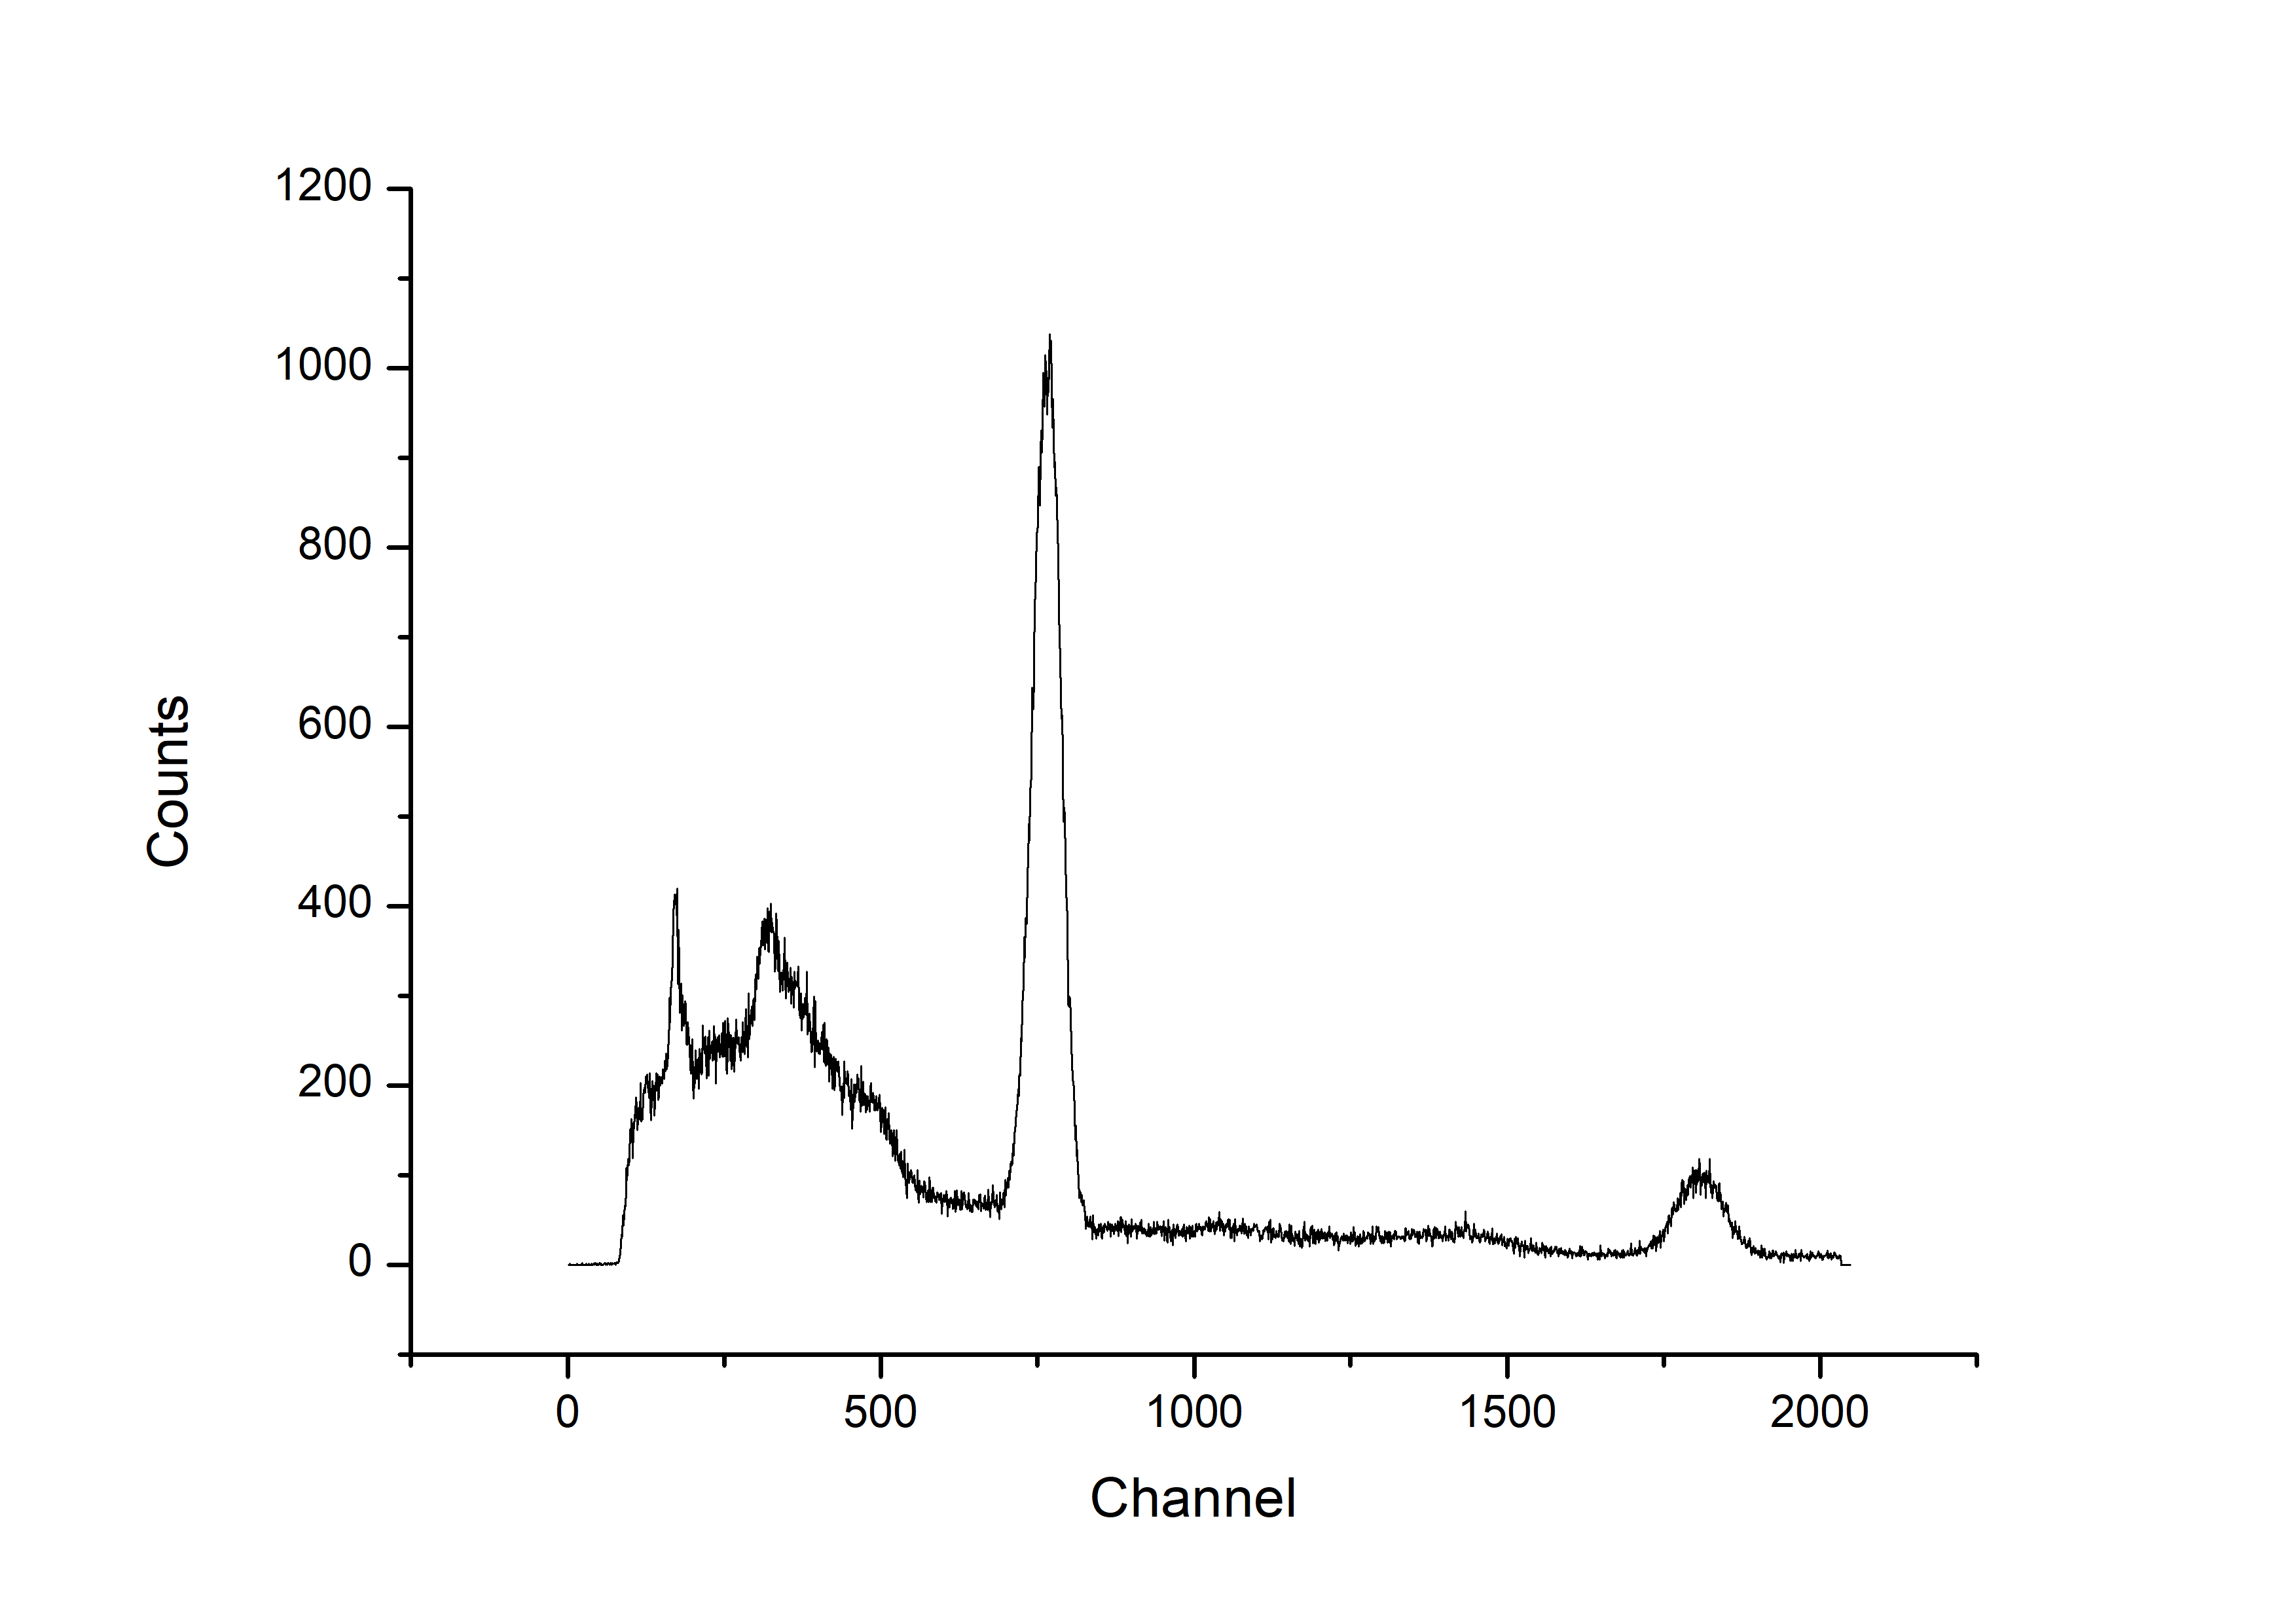
\includegraphics[width=1\linewidth]{Na.png}
\caption{Спектр $^{22}$Na} %% подпись к рисунку\label{ris:experimoriginal} %% метка рисунка для ссылки на него
\end{minipage}
\hfill 
\begin{minipage}[h]{0.48\linewidth}
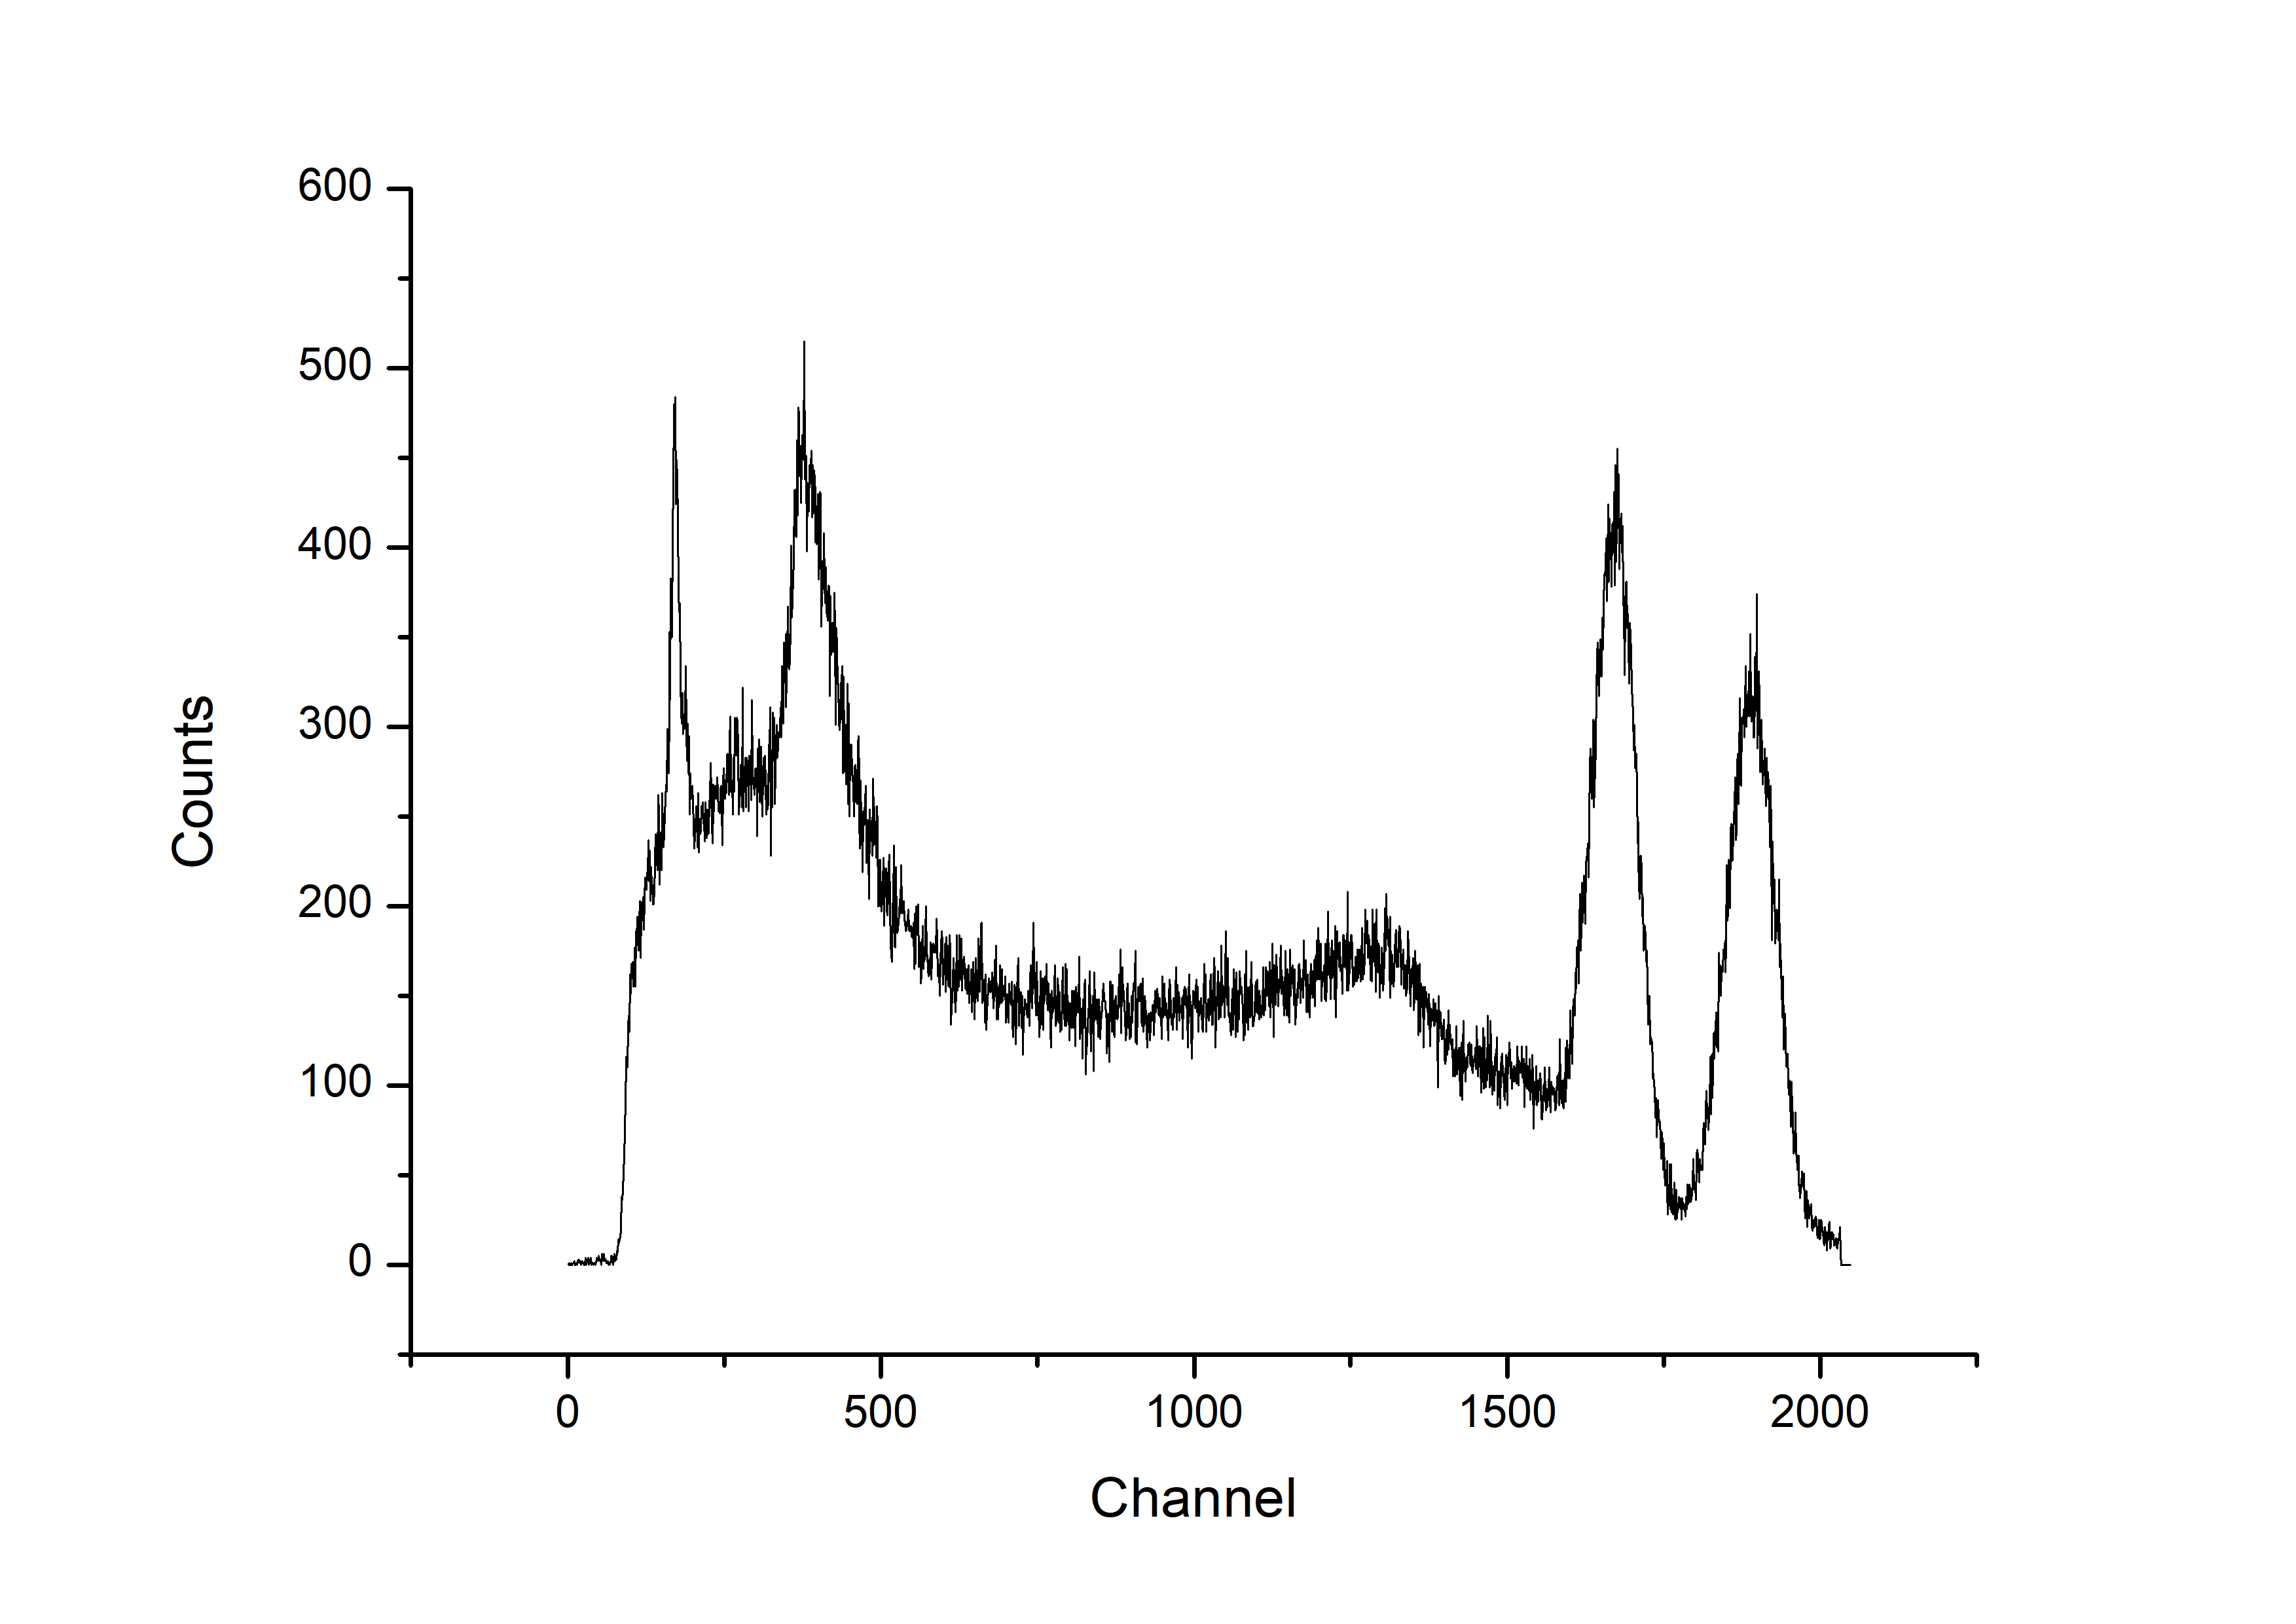
\includegraphics[width=1\linewidth]{Co.png}
\caption{Спектр $^{60}$Co}
\label{ris:experimcoded}
\end{minipage}
\end{center}
\end{figure}

        \begin{figure}[h]
\begin{center}
\begin{minipage}[h]{0.48\linewidth}
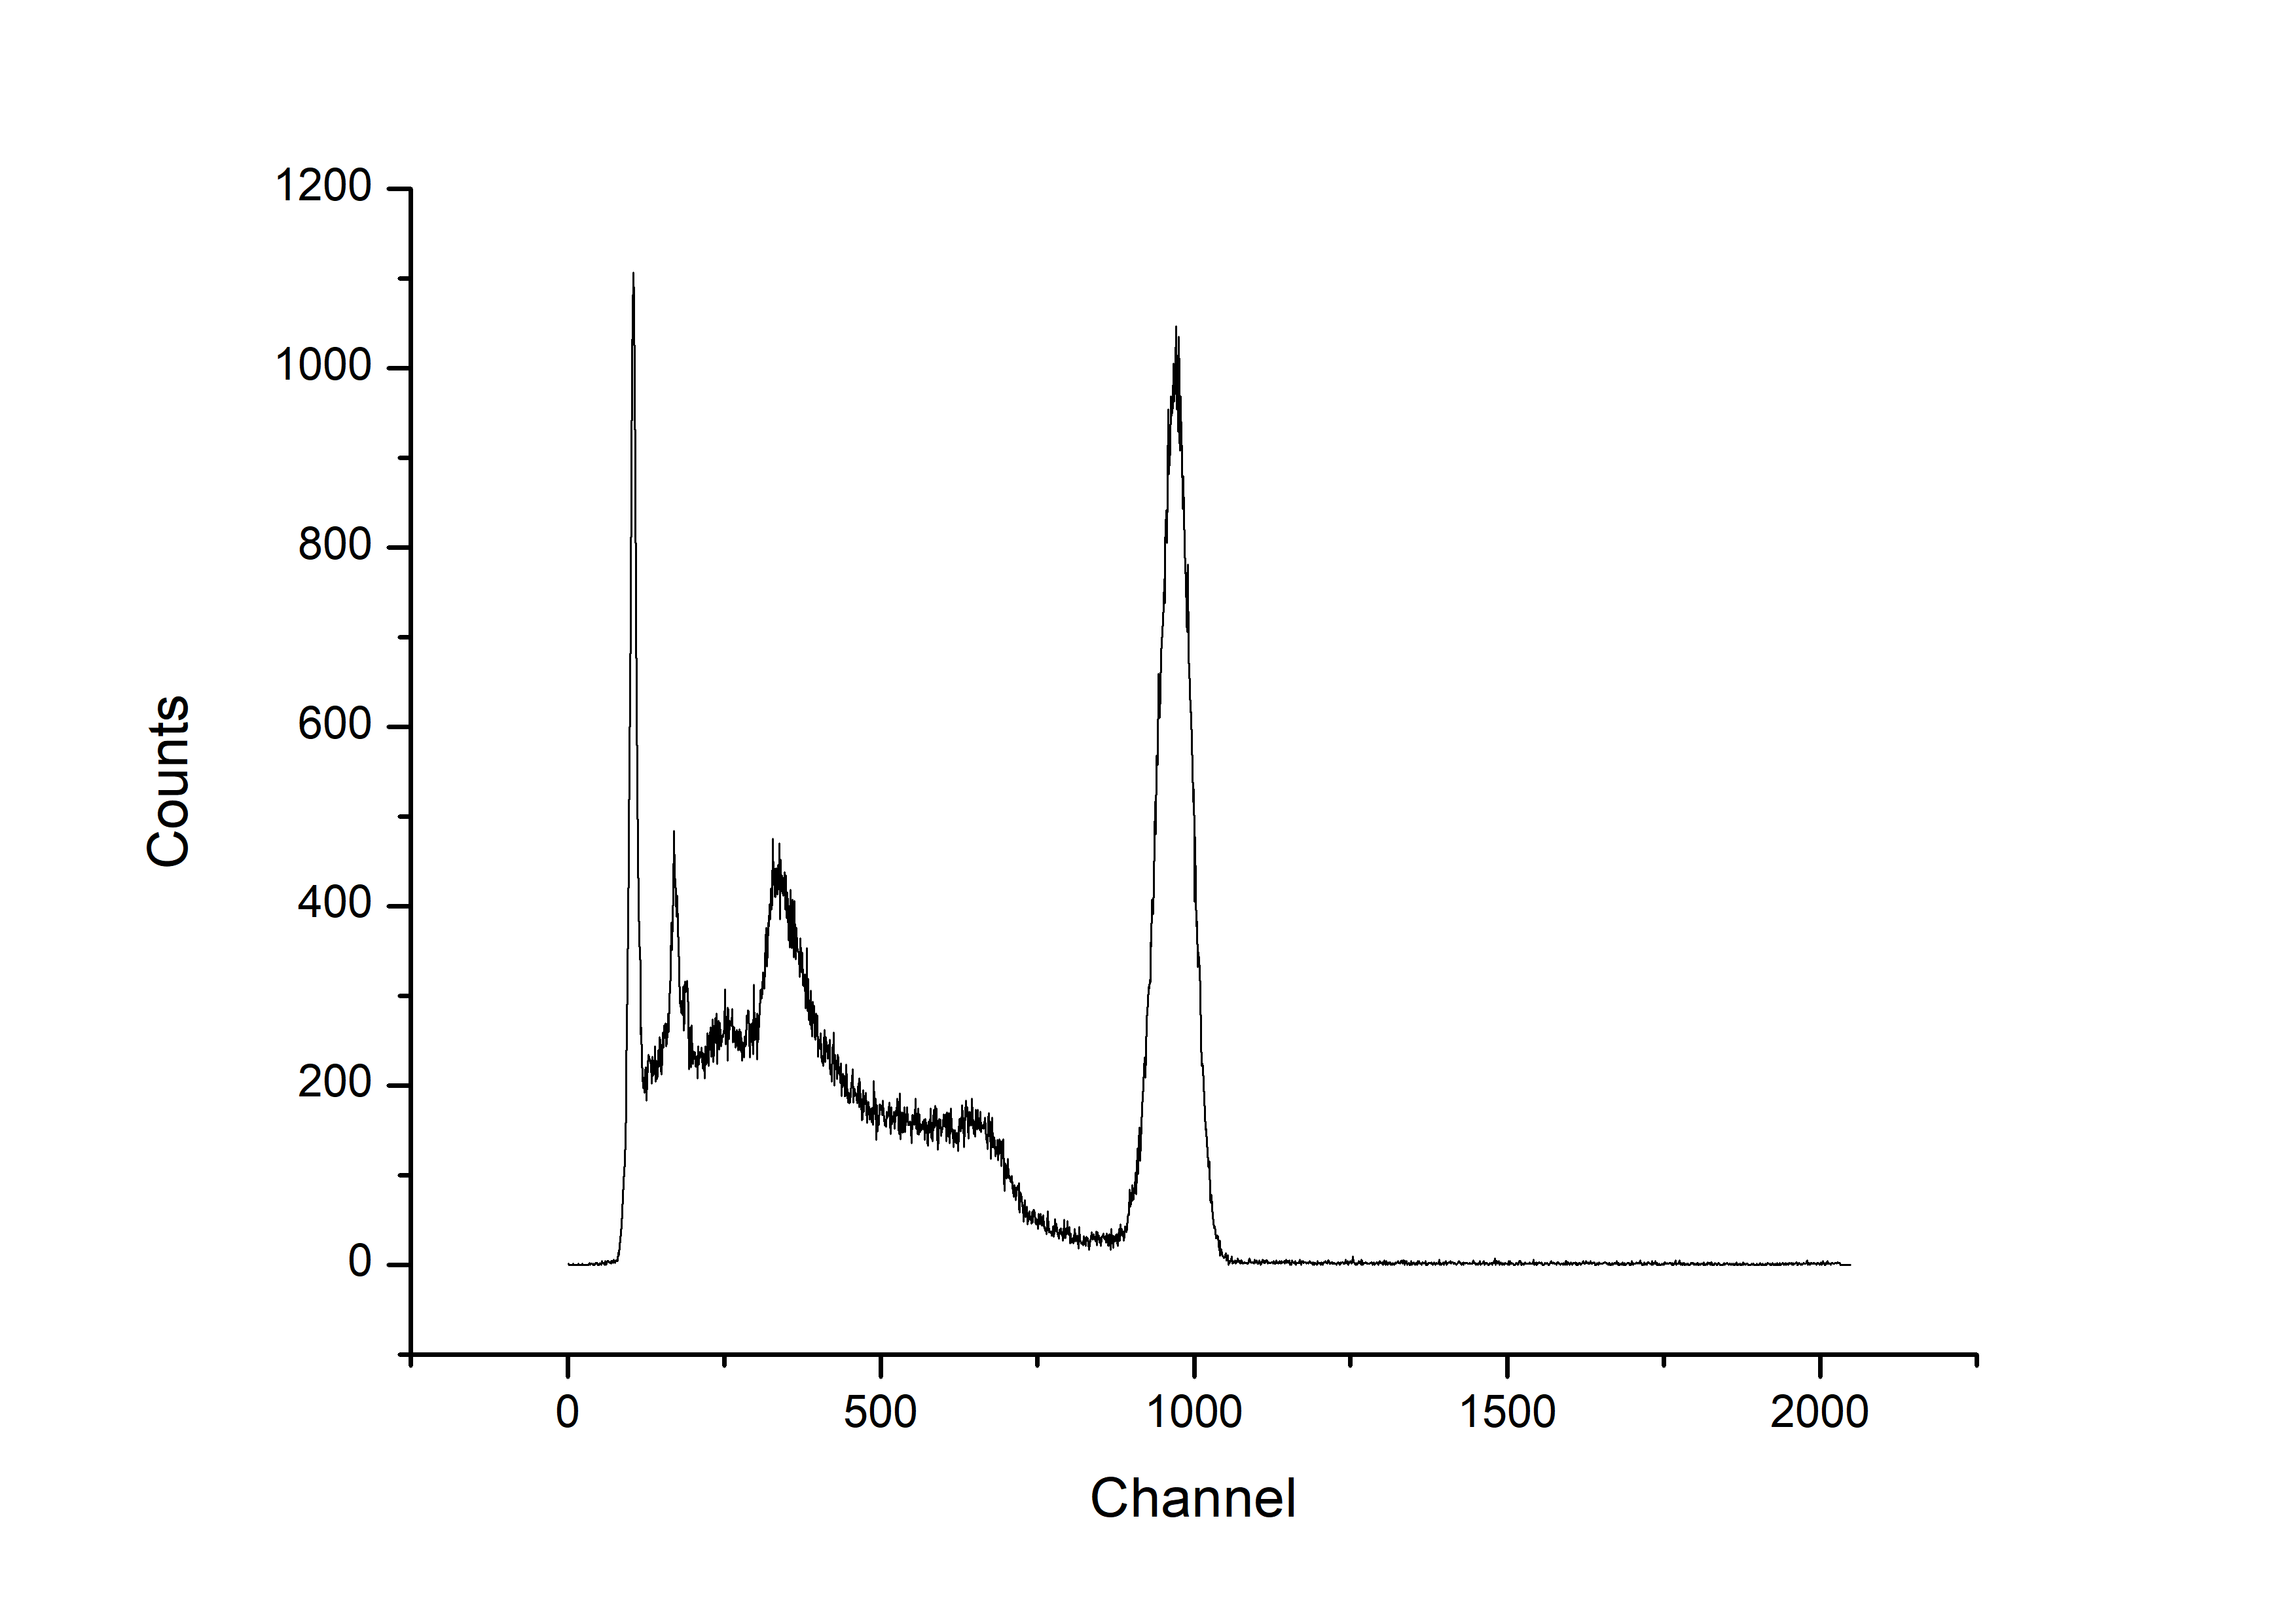
\includegraphics[width=1\linewidth]{Cs.png}
\caption{Спектр $^{137}$Cs} %% подпись к рисунку\label{ris:experimoriginal} %% метка рисунка для ссылки на него
\end{minipage}
\hfill 
\begin{minipage}[h]{0.48\linewidth}
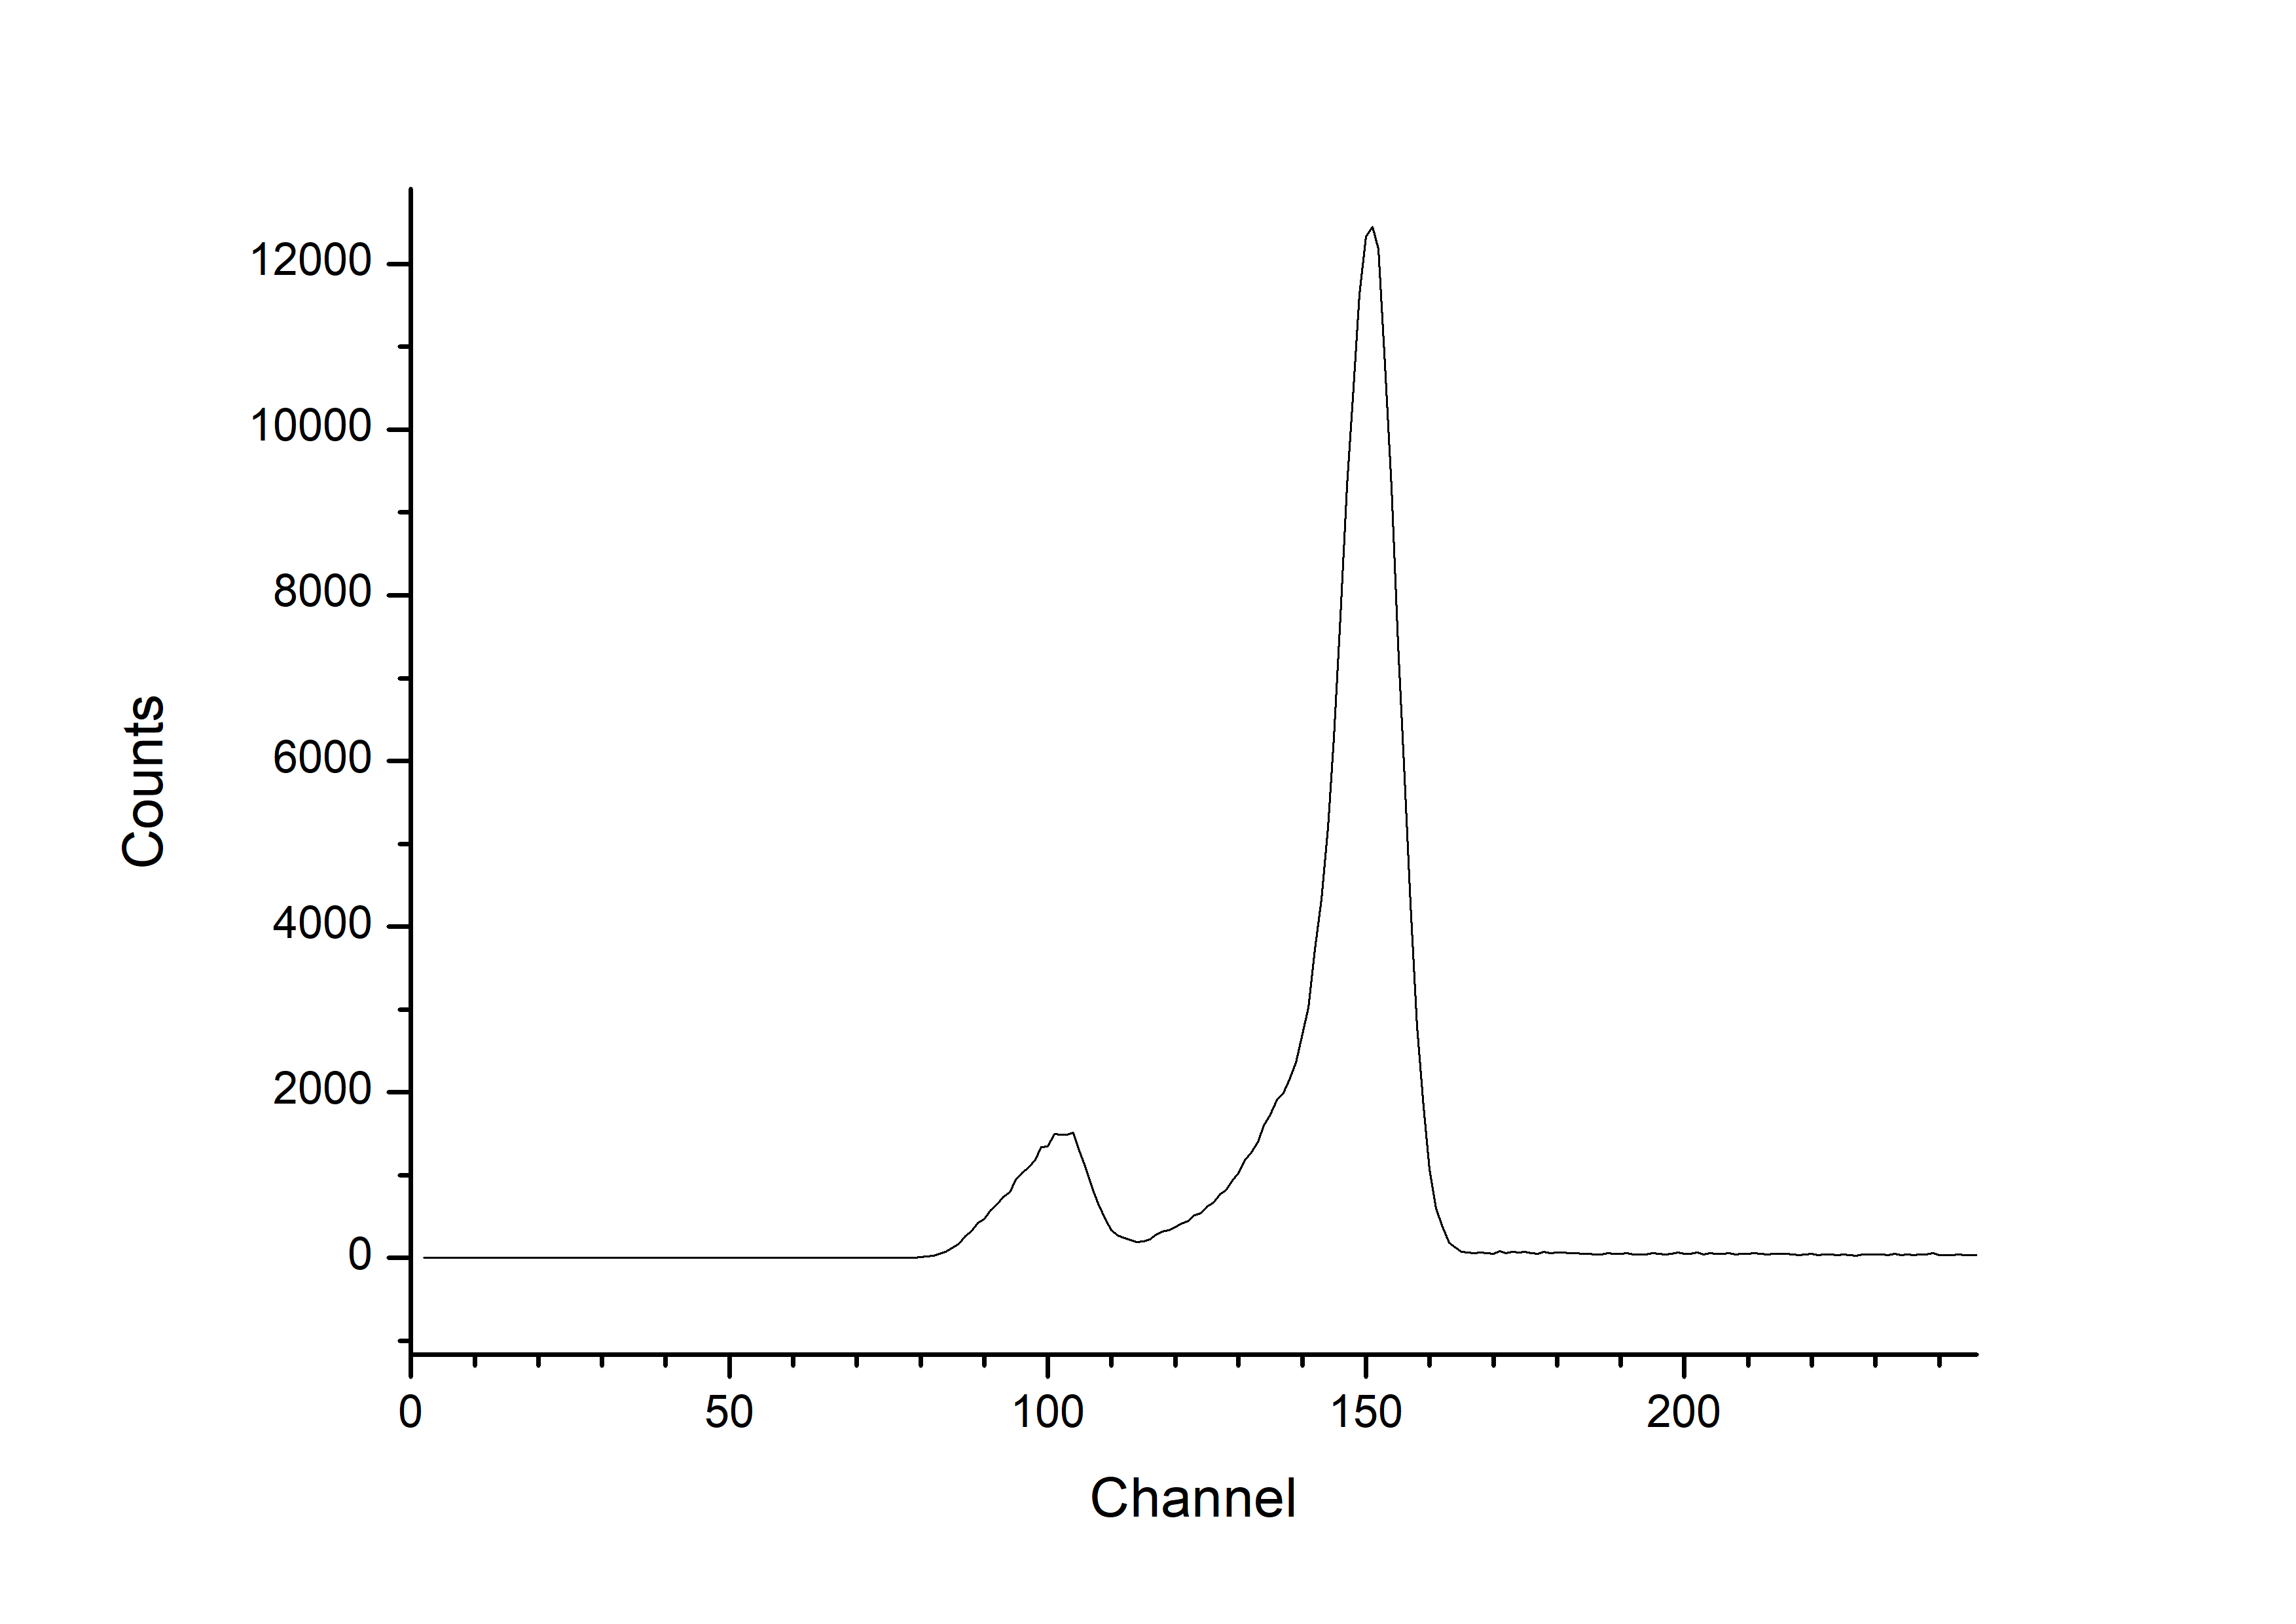
\includegraphics[width=1\linewidth]{Am.png}
\caption{Спектр $^{241}$Am}
\label{ris:experimcoded}
\end{minipage}
\end{center}
\end{figure}

        \begin{figure}[h]
\begin{center}
\begin{minipage}[h]{0.48\linewidth}
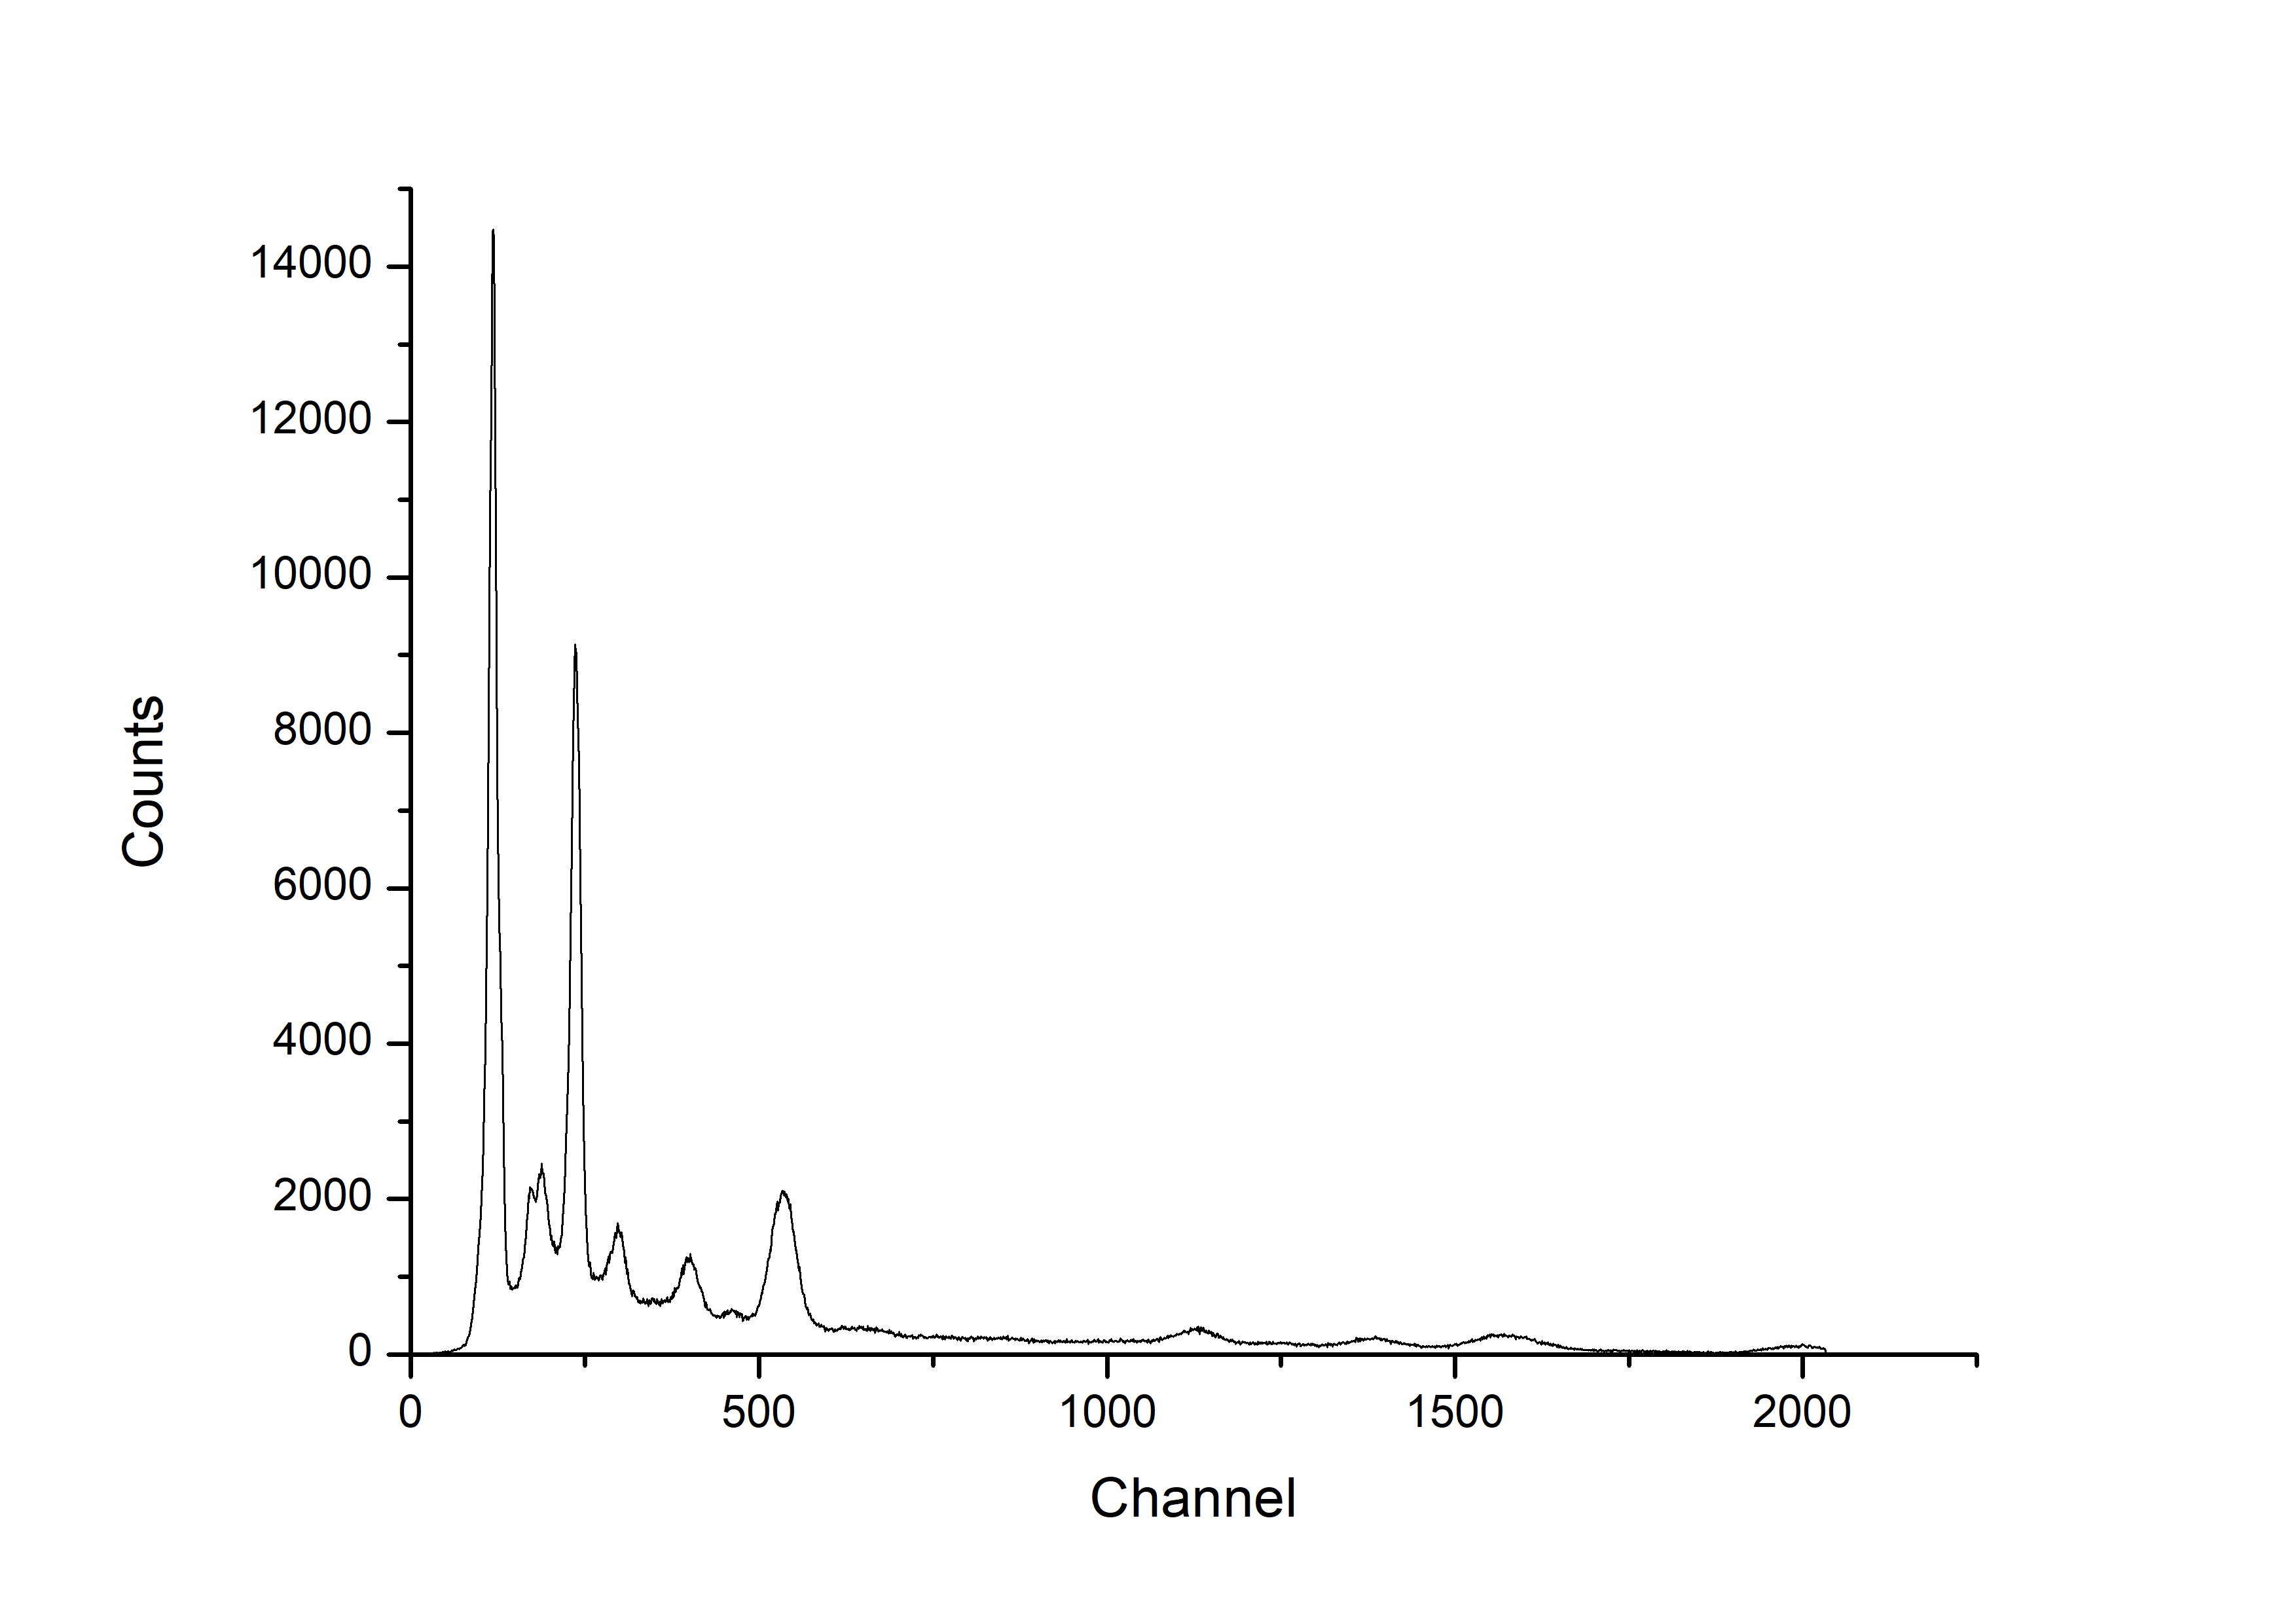
\includegraphics[width=1\linewidth]{Eu.png}
\caption{Спектр $^{152}$Eu} %% подпись к рисунку\label{ris:experimoriginal} %% метка рисунка для ссылки на него
\end{minipage}
\hfill 
\begin{minipage}[h]{0.48\linewidth}
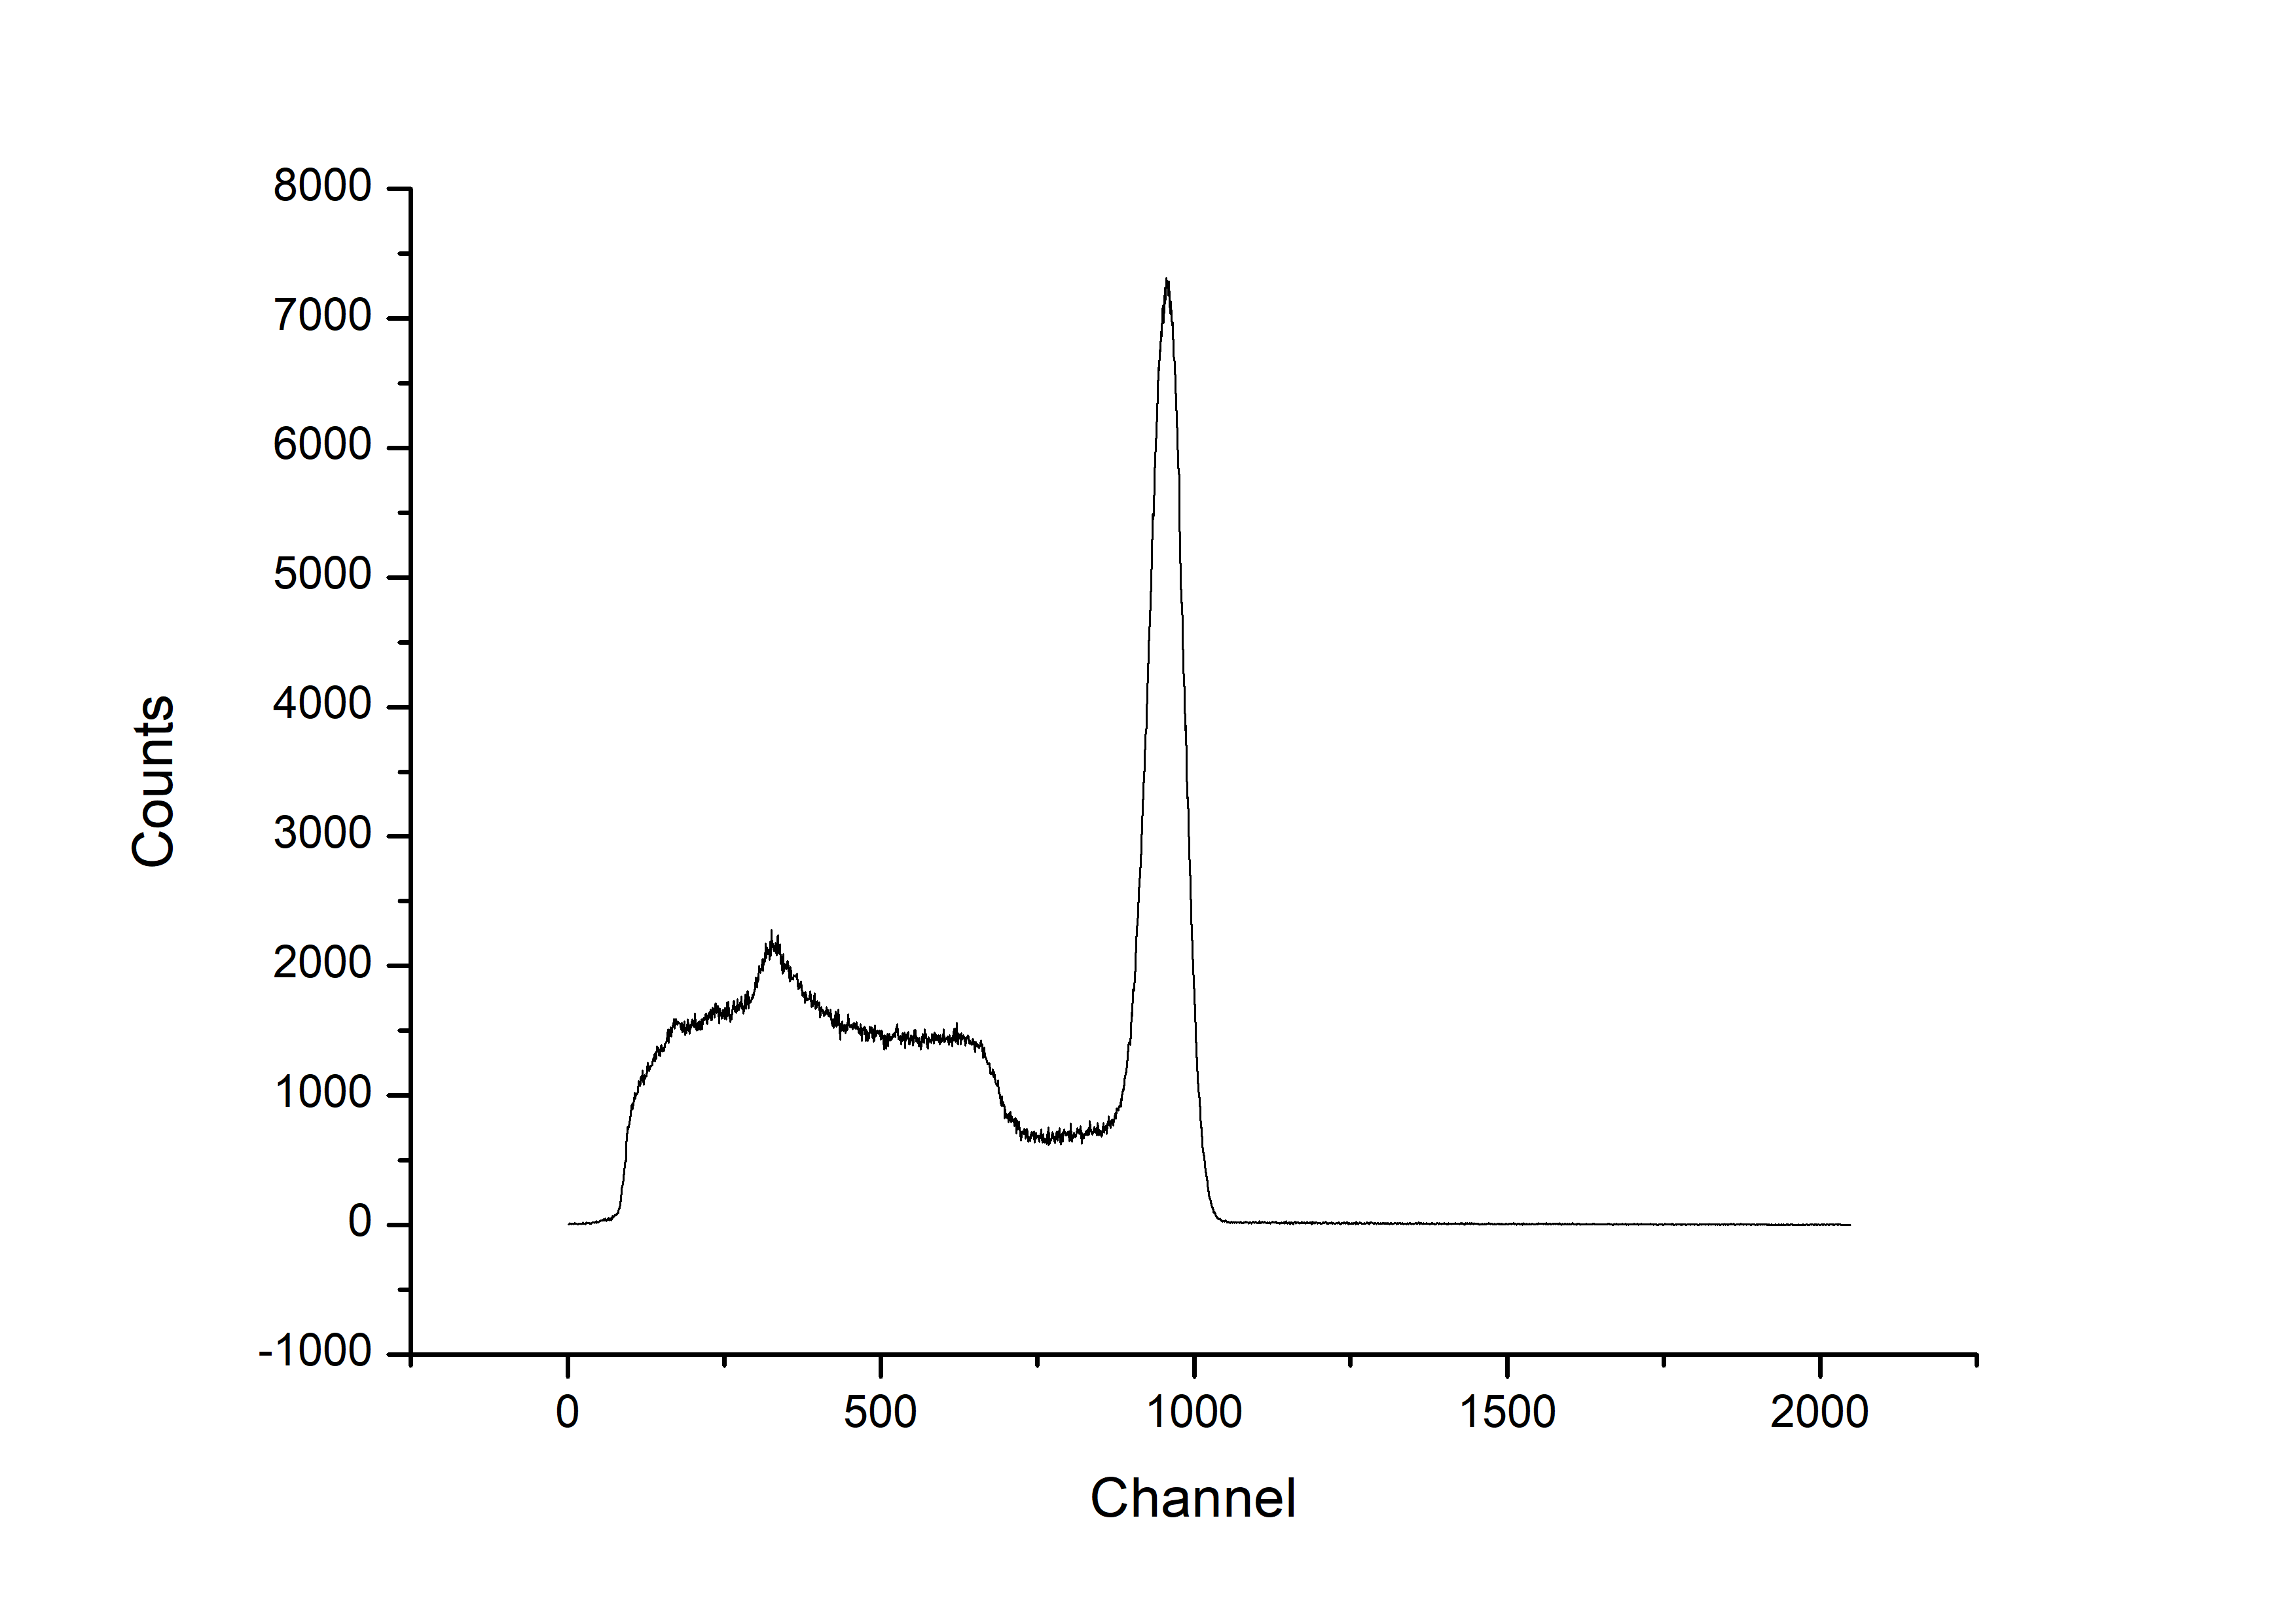
\includegraphics[width=1\linewidth]{Unknown.png}
\caption{Спектр неизвестного образца}
\label{ris:experimcoded}
\end{minipage}
\end{center}
\end{figure}

\begin{figure}[h]
\begin{center}
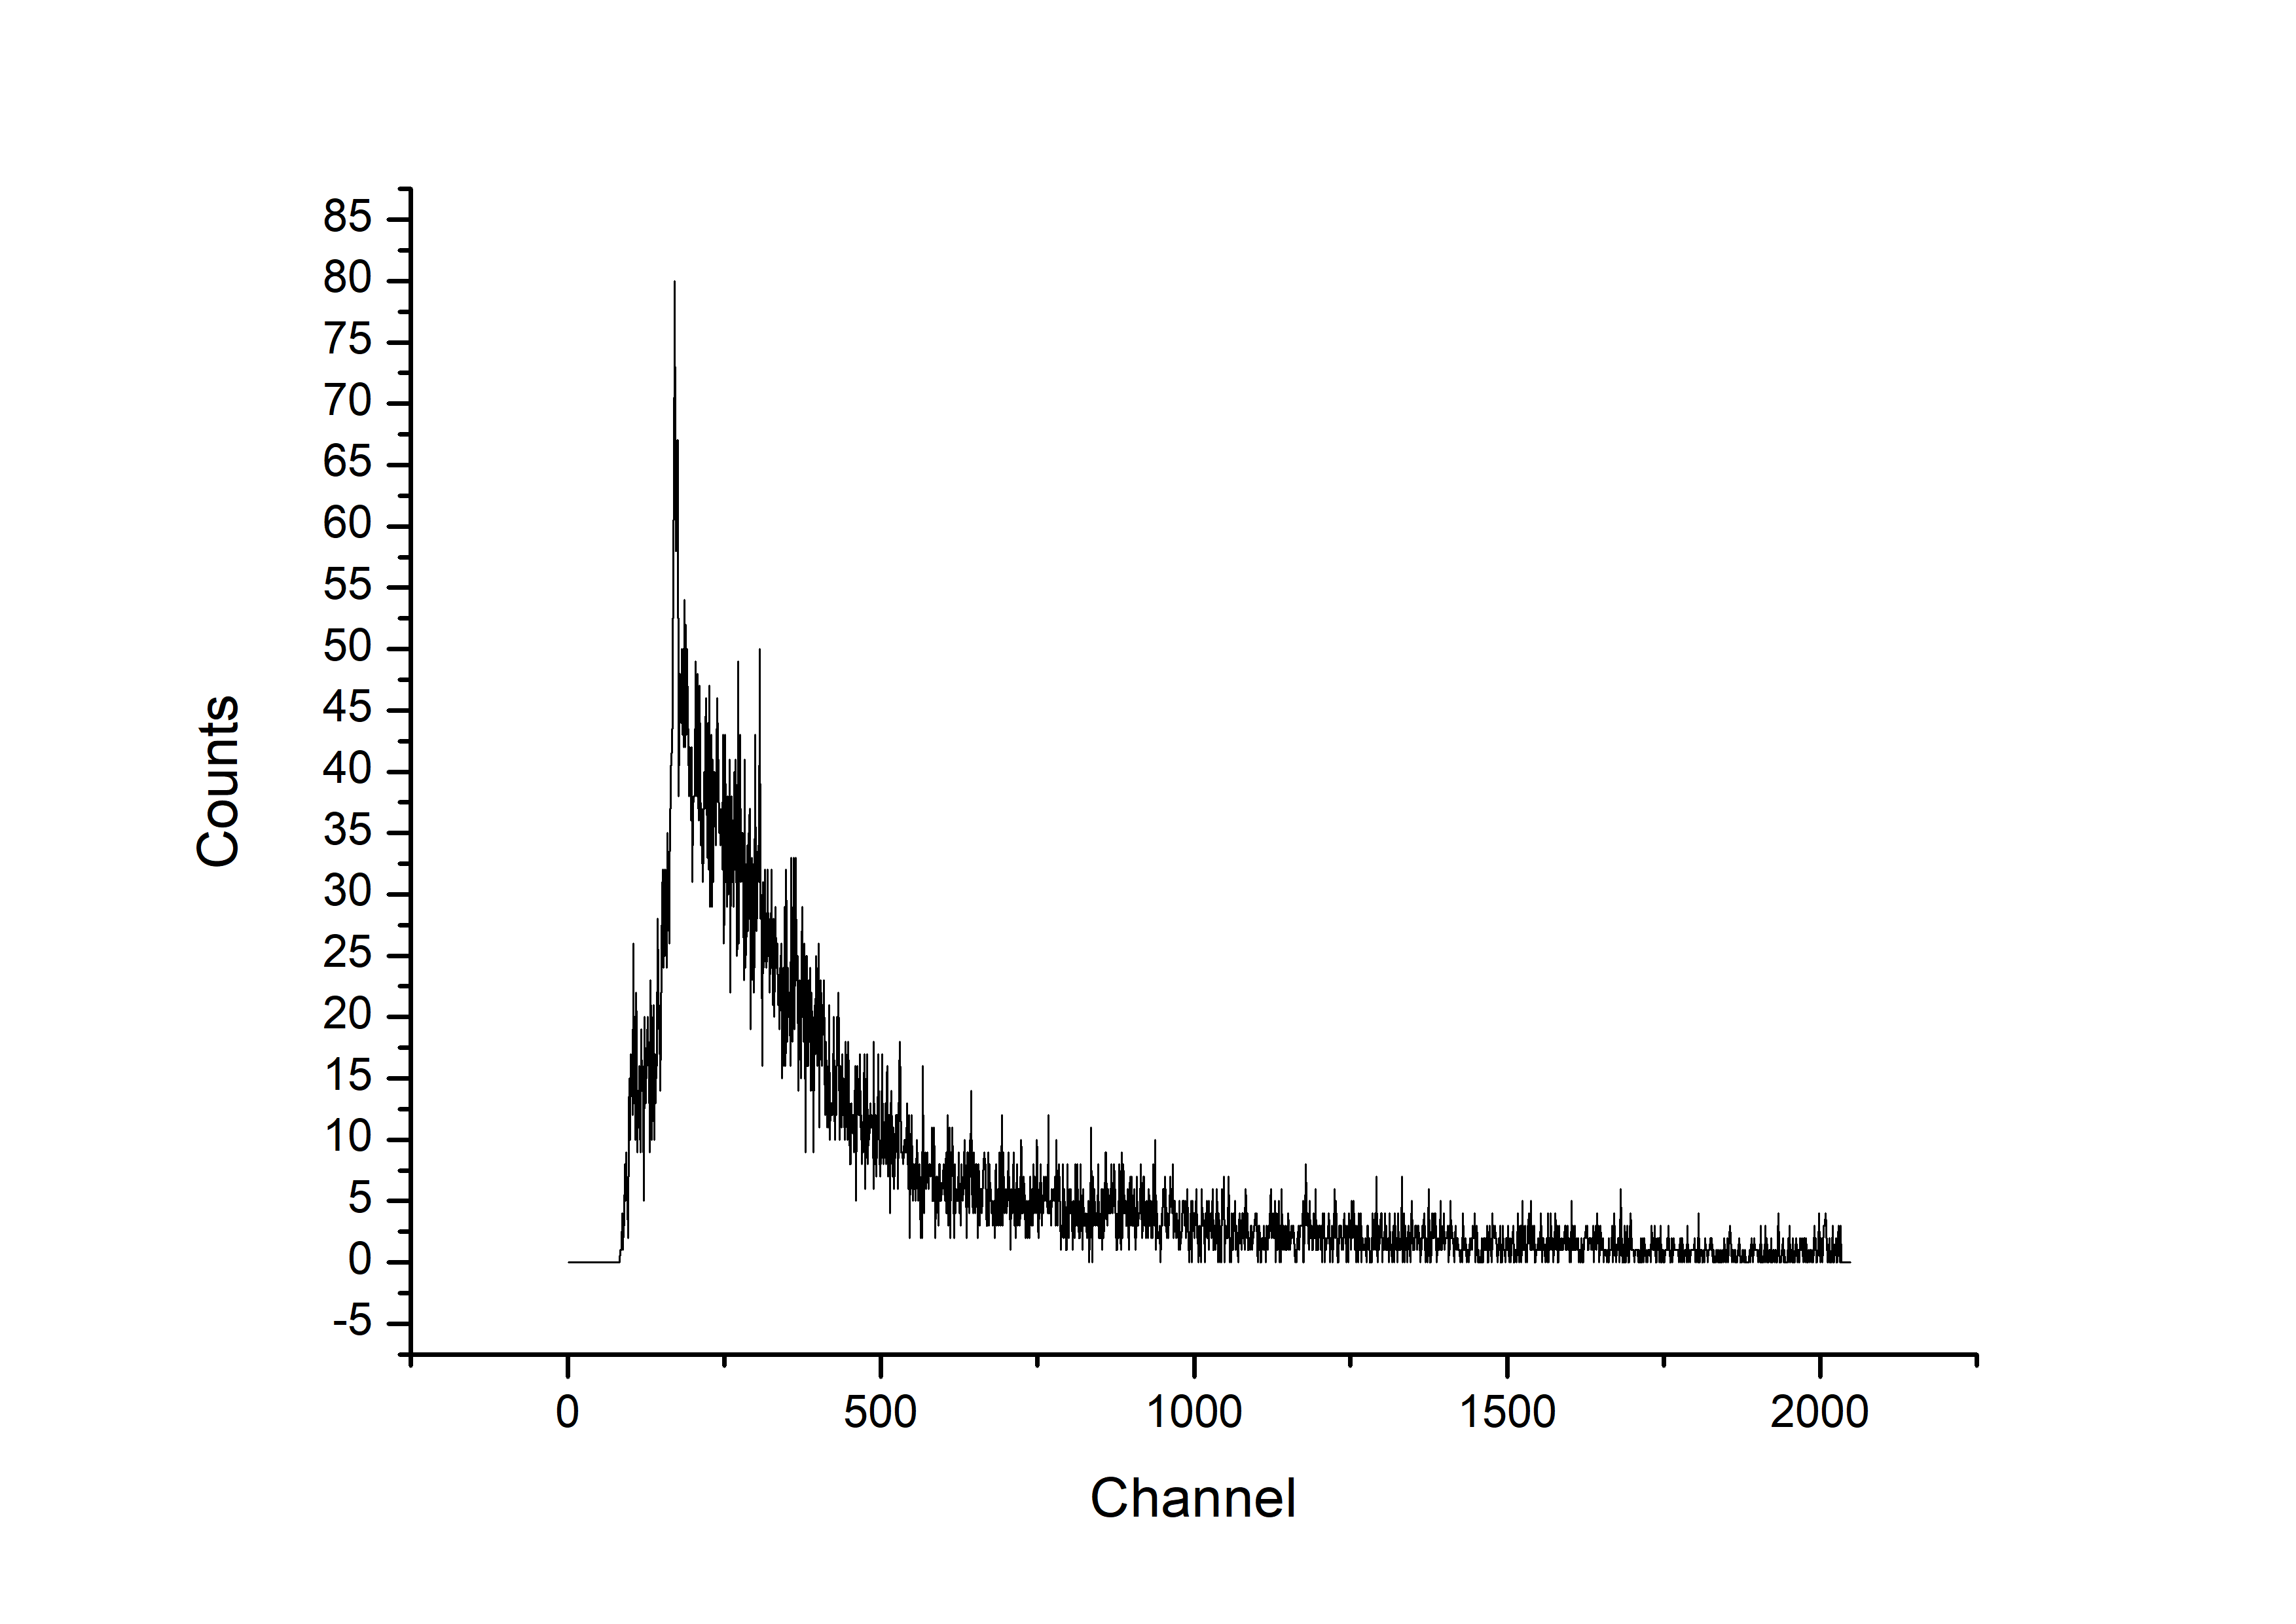
\includegraphics[width=0.48\linewidth]{background.png}
\caption{Спектр фона}
\label{ris:experimoriginal} %% метка рисунка для ссылки на него
\end{center}
\end{figure}

\clearpage

\item Используя известные значения пиков в спектрах натрия и цезия, построим калибровочный график соответствия номера канала определённому значению энергии (рис. 8). 
\begin{center}
    Пики натрия: \\
    511 кэВ - канал 766; \\
    661,7 кэВ - канал 971; \\
    Пик цезия:\\ 
    1275 кэВ - канал 1811 \\
\end{center}

\begin{figure}[h]
\begin{center}
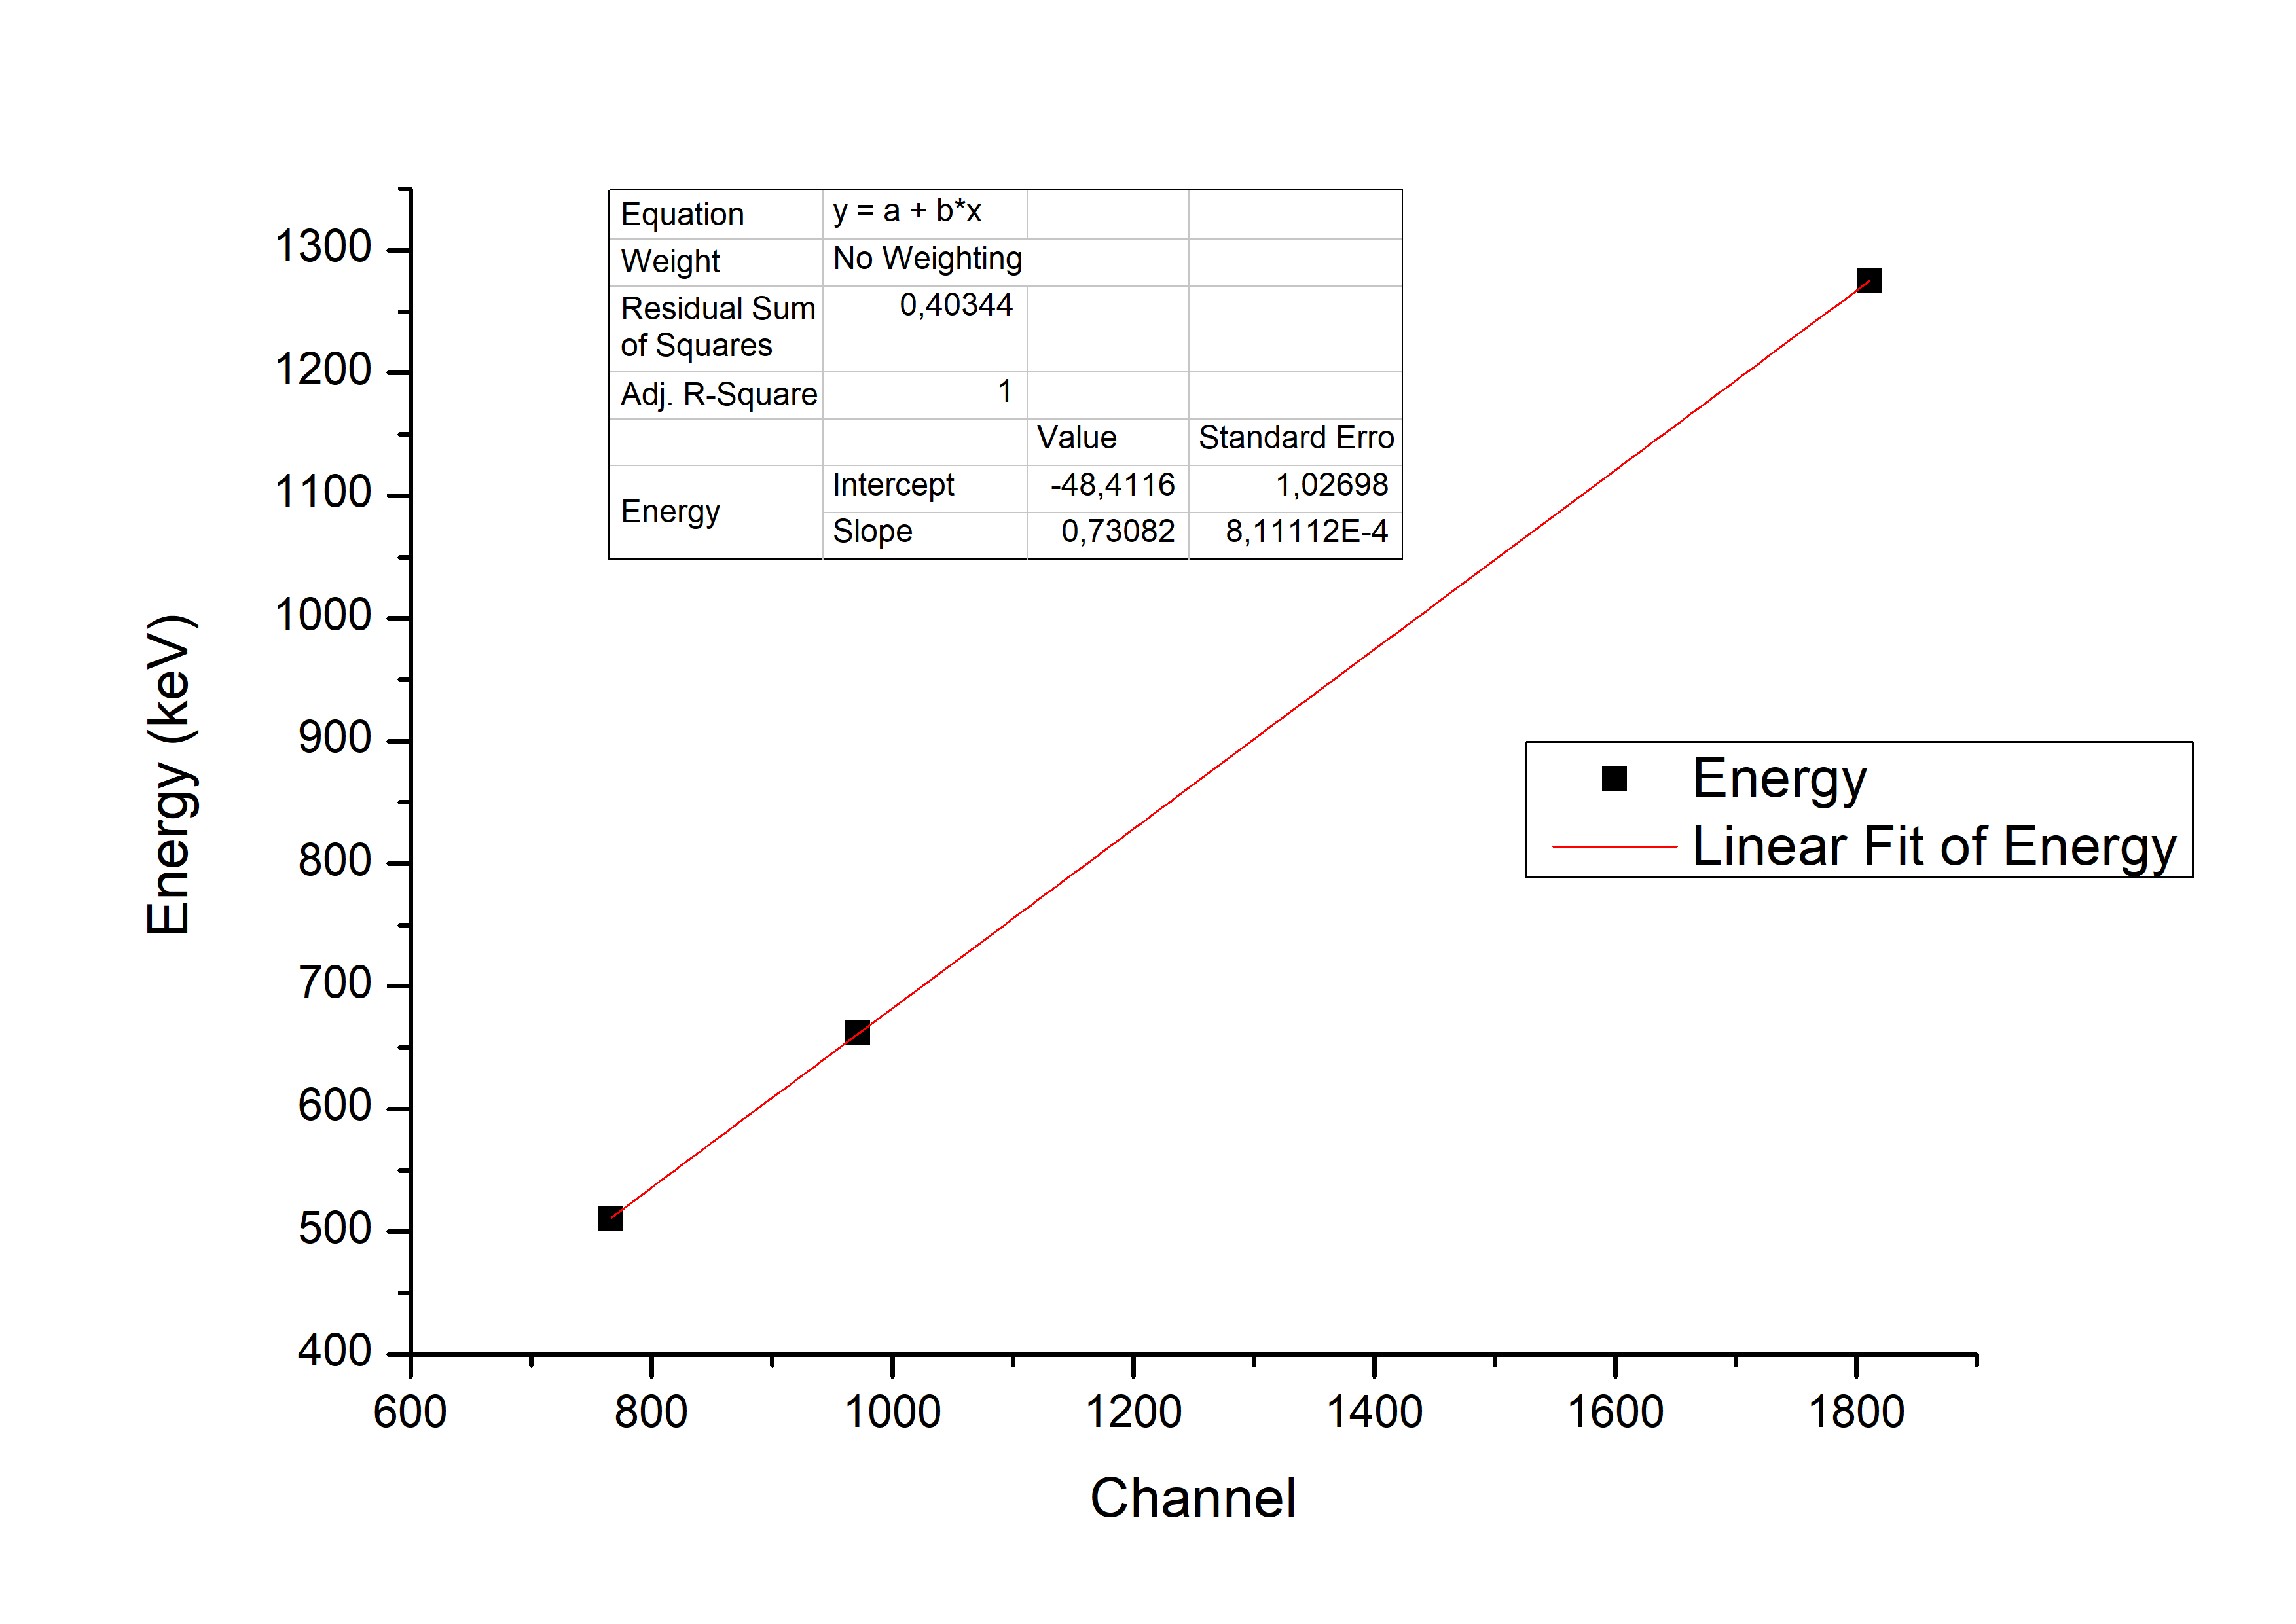
\includegraphics[width=12cm]{E(N).png}
\caption{Калибровочный график для перехода от номера канала к значению энергии}
\label{ris:experimoriginal} %% метка рисунка для ссылки на него
\end{center}
\end{figure}

Получаем уравнение для перехода от номера канала к значению энергии в кэВ:
\begin{center}
    $E = 0.73N_i - 48,41$
\end{center}

\item Используя калибровочный график, определим для всех остальных источников значения энергии пиков полного поглощения $E_i$ , их ширины на половине высоты $\triangle E_i$ и энергетическое разрешение $R_i$ . Результаты занесём в таблицу 1. В последний столбец занесём справочные значения для соответствующих энергий пиков полного поглощения (знаком (к) отмечены значения, по которым проводилась калибровка значений прибора)

    \begin{table}[h]
    \centering
    \begin{center}
    \caption{Пики полного поглощения различных образцов}
    \end{center}
    \vspace{0.1cm}
    \label{tab:my_label}
    \begin{tabular}{|p{1.5cm}|p{1.5cm}|p{1.5cm}|p{1.5cm}|p{1.6cm}|p{1.5cm}|p{1.5cm}|}
\hline
  Элемент & $N_i$ & $\triangle N_i$ & $E_i$, MeV & $\triangle E_i$, MeV & $R_i$ & $E$, MeV \\
 \hline
 $^{22}$Na & 1811 & 83 & 1.274 & 0.030 & 0.023 & 1.274 (к) \\
\hline
 $^{60}$Co & 1670 & 37 & 1.171 & 0.027 & 0.023  & 1.173 \\
\hline
 $^{60}$Co & 1892 & 45 & 1.333 & 0.033 & 0.024 & 1.332 \\
\hline
$^{137}$Cs & 967 & 62 & 0.662 & 0.022 & 0.032 & 0.662 (к) \\
\hline
$^{241}$Am & 149 & 13 & 0.060 & 0.004 & 0.067 & 0.595 \\
\hline
$^{152}$Eu & 235 & 17 & 0.123 & 0.006 & 0.045 & 0.122 \\
\hline
$^{152}$Eu & 399 & 31 & 0.243 & 0.010 & 0.040 & 0.245 \\
\hline
$^{152}$Eu & 534 & 41 & 0.341 & 0.015 & 0.041 & 0.344 \\
\hline
 \end{tabular}
\end{table} 

\item Исследуем спектр неизвестного образца (рис. 9). Для этого вынем сцинтиллятор из установки и снимем спектр непосредственно в трубке с образцом. Построим на одном графике спектры цезия и неизвестного образца - можно легко убедиться, что пик полного поглощения у них практически совпадает. Делаем вывод, что исследуемый образец - это $^{137}$Cs.
\begin{figure}[h]
\begin{center}
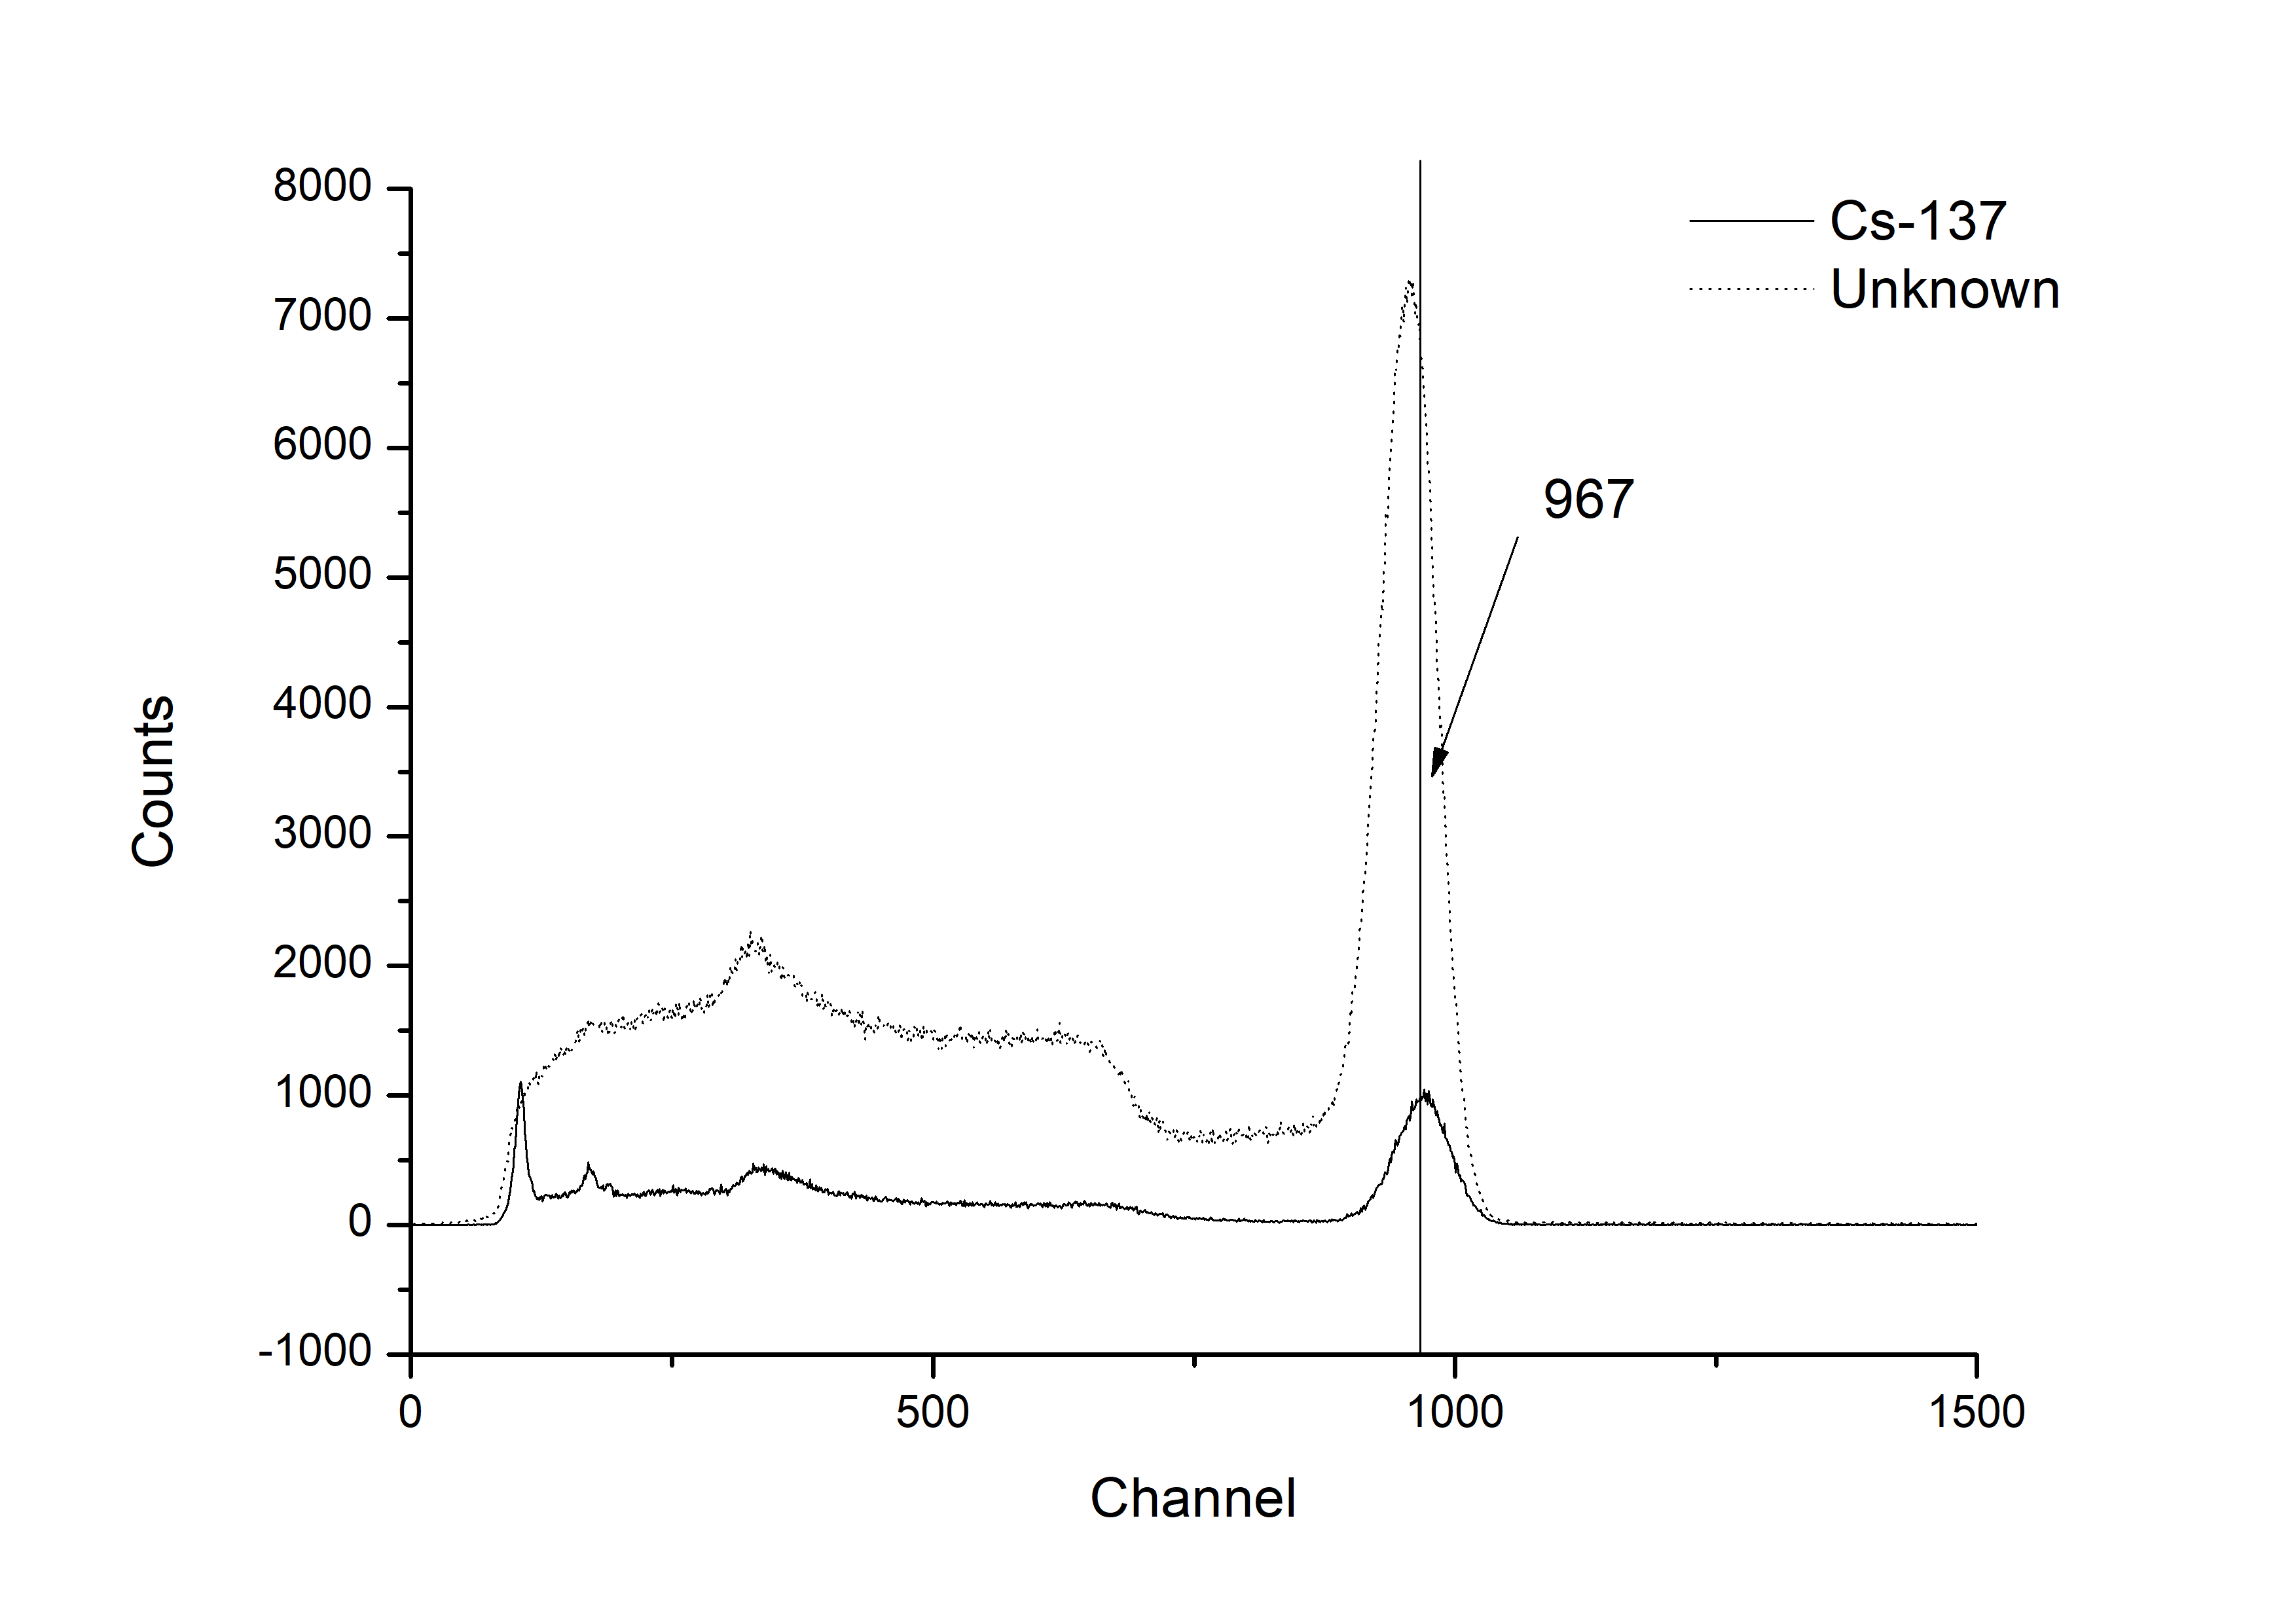
\includegraphics[width=12cm]{Cs+unknown.png}
\caption{Спектры $^{137}$Cs и неизвестного образца}
\label{ris:experimoriginal} %% метка рисунка для ссылки на него
\end{center}
\end{figure}

\item По графикам определим энергию характеристического излучения свинца, служащего защитой спектрометра от внешнего излучения. На всех спектрах, кроме спектра неизвестного образца, снятого вне установки, в той или иной степени выражена спектральная линия, соответствующая энергии 75 keV. Эта энергия и есть энергия характеристического излучения свинца.


\item Проверим зависимость (6). Для этого построим график зависимости $R^2 = f(1/E)$ (рис. 10). Наблюдается линейная зависимость. Из-за неточностей в определении полуширины пиков точки не лежат на одной прямой. 

\begin{figure}[h]
\begin{center}
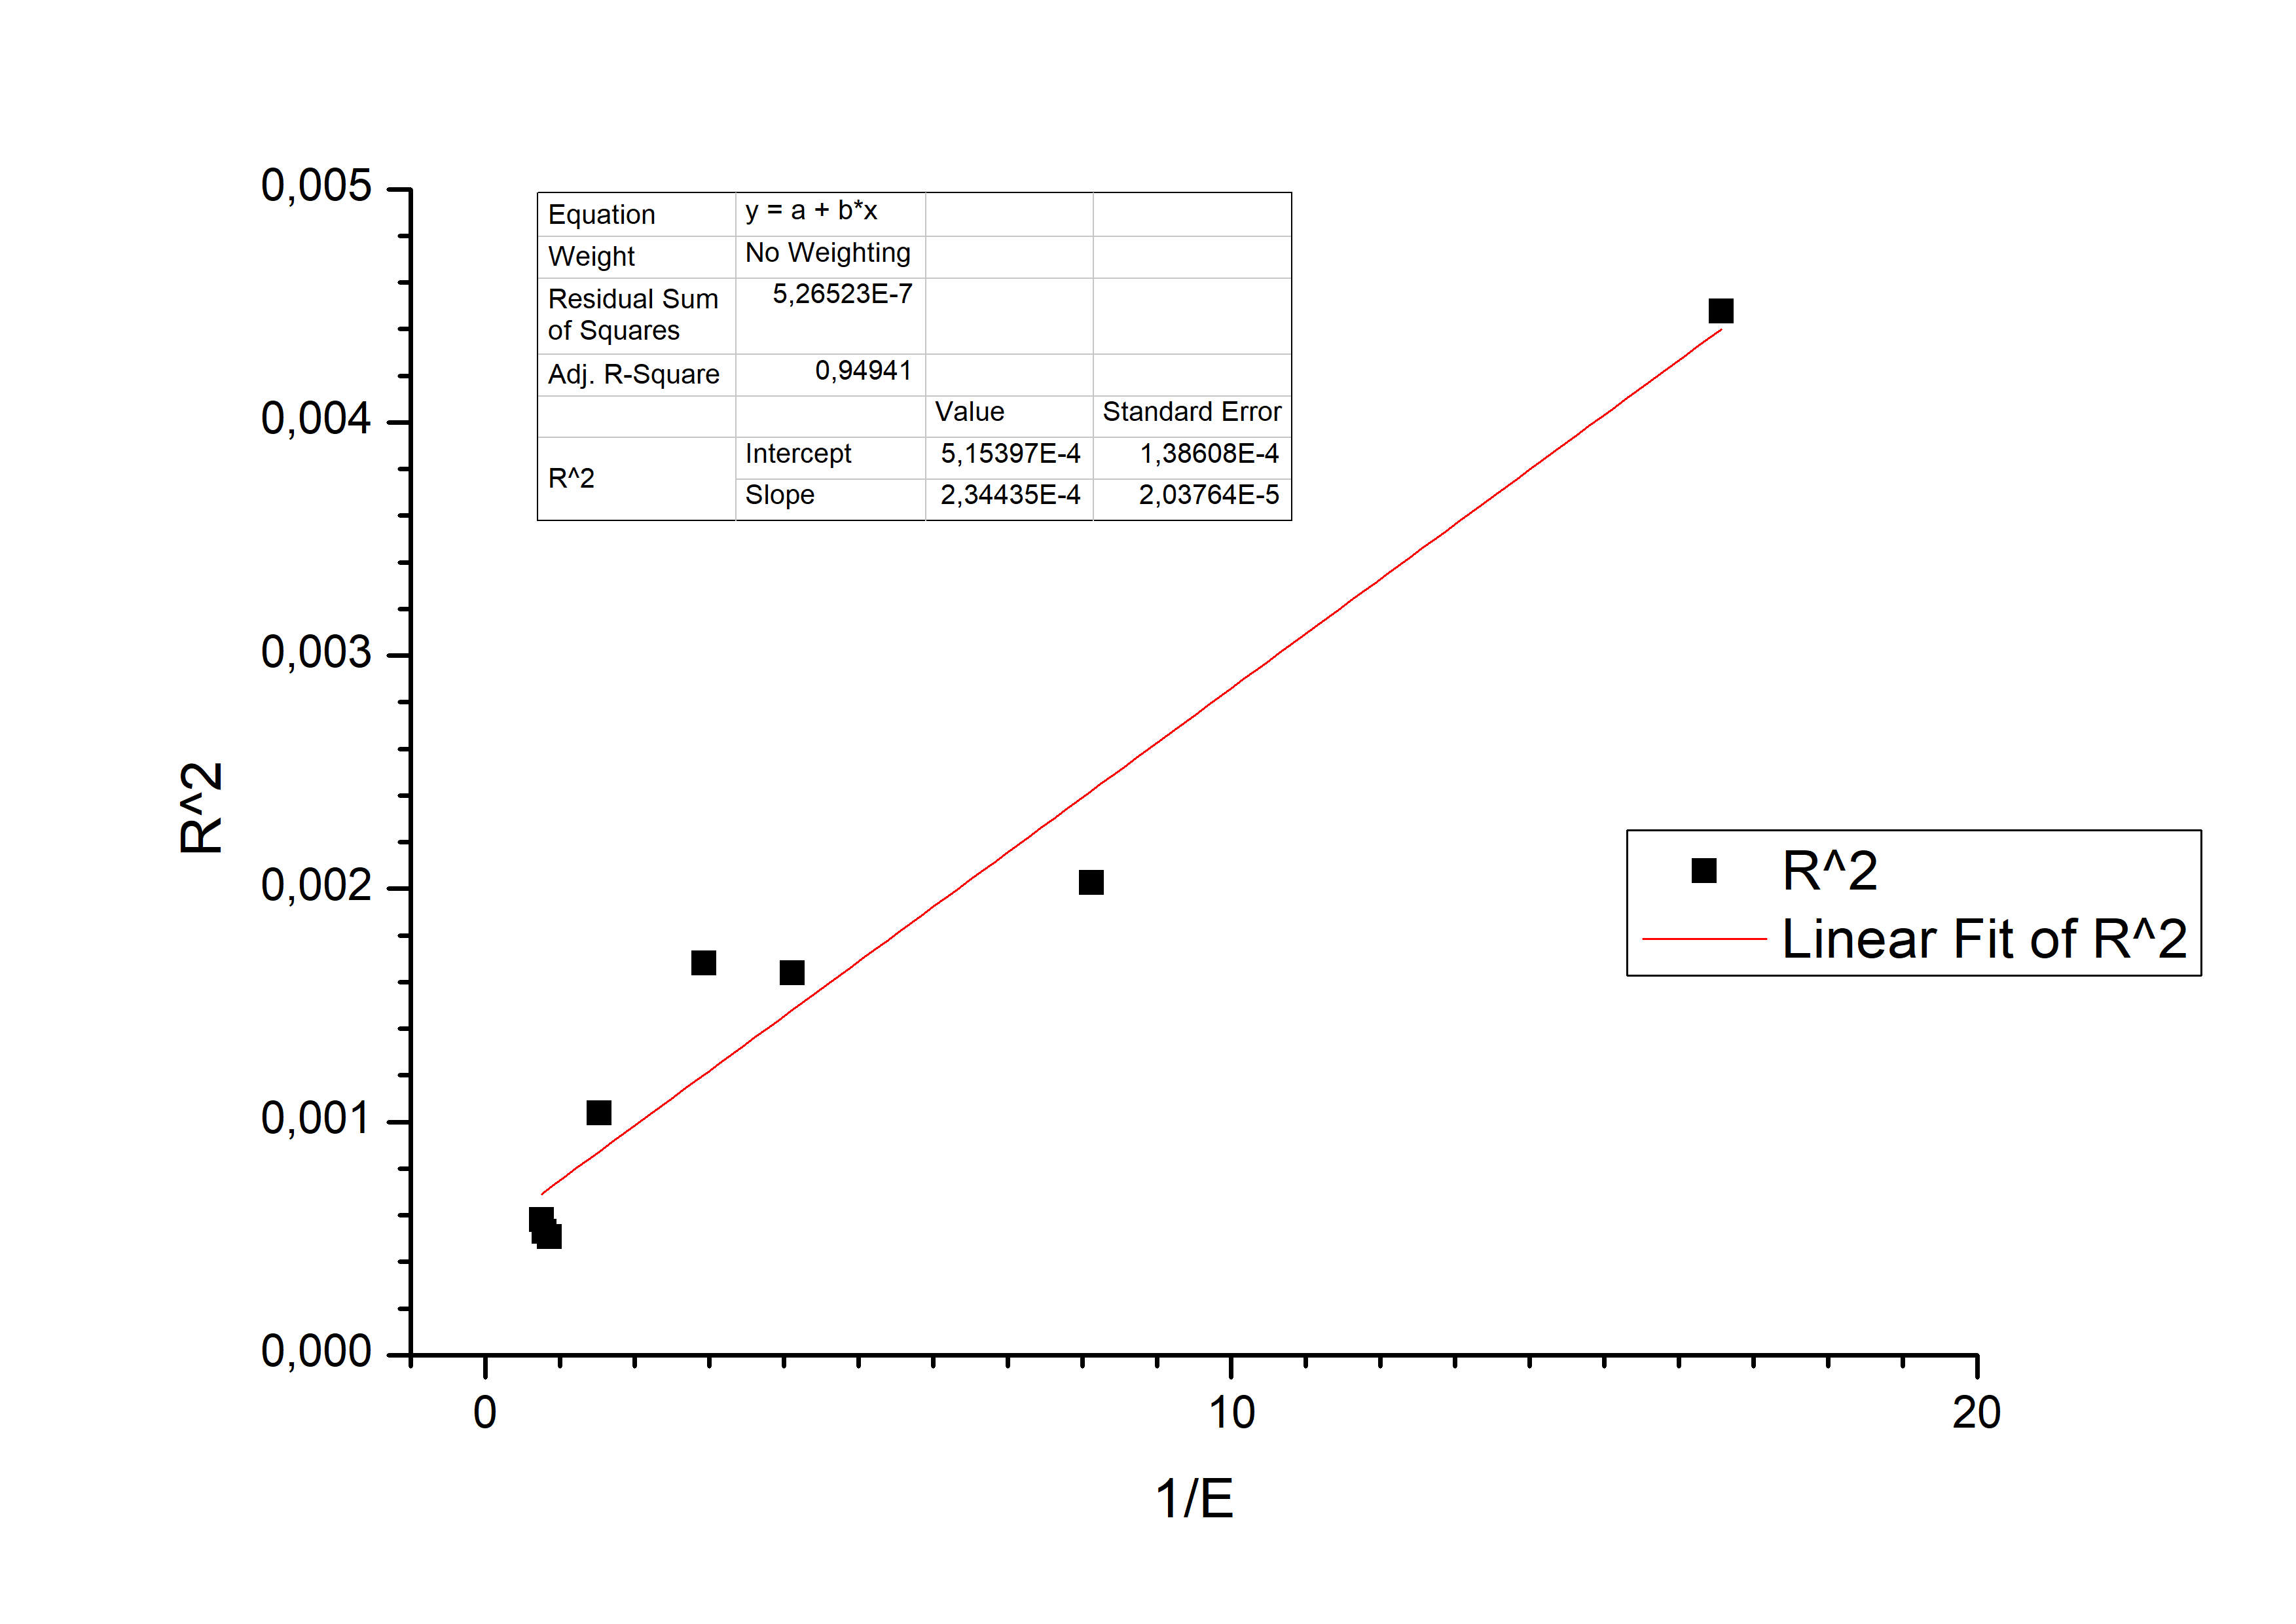
\includegraphics[width=12cm]{R.png}
\caption{График зависимости $R^2$ от $1/E$}
\label{ris:experimoriginal} %% метка рисунка для ссылки на него
\end{center}
\end{figure}

\item Определим энергии края комптоновского поглощения для образцов $^{22}$Na, $^{137}$Cs, $^{60}$Co, сравним их с соответствующими справочными значениями.
\begin{center}
  $^{60}$Co \hspace{1cm} $E_C_{exp} = 0,922$ MeV \hspace{1cm} $E_C_{th} = 0.963$ MeV \\
$^{137}$Cs \hspace{1cm} $E_C_{exp} =0,448$ MeV \hspace{1cm} $E_C_{th} = 0.477$ MeV \\
$^{22}$Na \hspace{1cm} $E_C_{exp} =0,999$ MeV \hspace{1cm} $E_C_{th} = 1.062$ MeV \\
 \end{center}

\item В спектрах, где наблюдаются пики обратного рассеяния, определим энергии этих пиков и сравним измеренные значения с определёнными по формуле (2)
\begin{center}
    $E_b_s = \frac{E_{\gamma}}{1 + \frac{2E_{\gamma}}{m_e c^2}}$
\end{center}

\begin{center}
  $^{60}$Co ($E = 1.171$ MeV) \hspace{1cm} $E_C_{exp} = 0,228$ MeV \hspace{1cm} $E_C_{th} = 0.209$ MeV \\
    $^{60}$Co ($E = 1.333$ MeV)\hspace{1cm} $E_C_{exp} = 0,228$ MeV \hspace{1cm} $E_C_{th} = 0.214$ MeV \\
$^{137}$Cs ($E = 0.662$ MeV)\hspace{1cm} $E_C_{exp} =0,198$ MeV \hspace{1cm} $E_C_{th} = 0.184$ MeV \\
\end{center}

Эти значения практически совпадают. Пики обратного рассеяния в спектре кобальта, отвечающие разным пикам полного поглощения, на графике неразрешимы (виден один широкий пик).

\end{enumerate}

\section{Вывод}

В ходе работы после калибровки прибора были сняты спектры образцов $^{22}$Na,  $^{60}$Cо,  $^{137}$Cs, $^{241}$Am, $^{152}$Eu, а также исследован спектр неизвестного образца и определен его состав ($^{137}$Cs). В спектрах были исследованы пики, соответствующие следующим взаимодействиям гамма-квантов с веществом:
\begin{itemize}
    \item фотоэффект (пики полного поглощения)
    \item эффект Комптона (характерное распределение энергий в спектре, оканчивающееся комптоновским краем)
    \item обратное рассеяние (пики обратного рассеяния)
    \item аннигиляция позитронов (пик 511 keV в спектре натрия, по которому проводилась калибровка)
\end{itemize}

Все значения энергии, опеределённые по спектрам, практически совпадали с табличными и расчётными. \par

Также была проверена линейная зависимость квадрата спектрального разрешения прибора от величины, обратной энергии полного поглощения.

\end{document}
